% !TEX root = ../../main.tex

\subsection{Characterisation of trends}\label{def:trends}

The graphs in \autoref{def:fgr:tga-defects} summarize the 
trends in missing linker defects as calculated through 
the TGA plateau at \SI{420}{\degreeCelsius}. The DMF leached samples,
due to the multiple datapoints with different acid concentrations
show the clearest influence of this variable on defect
generation. Even small amounts of modulator leads to the decrease of 
the linker-to-node ratio, but the increase in concentration stops 
having an effect at around 20:1 equivalents. It is likely that
the trends are similar with other solvents, even if less 
datapoints are available.

\begin{figure}[htb]
    \centering

    \begin{subfigure}{0.25\linewidth}
        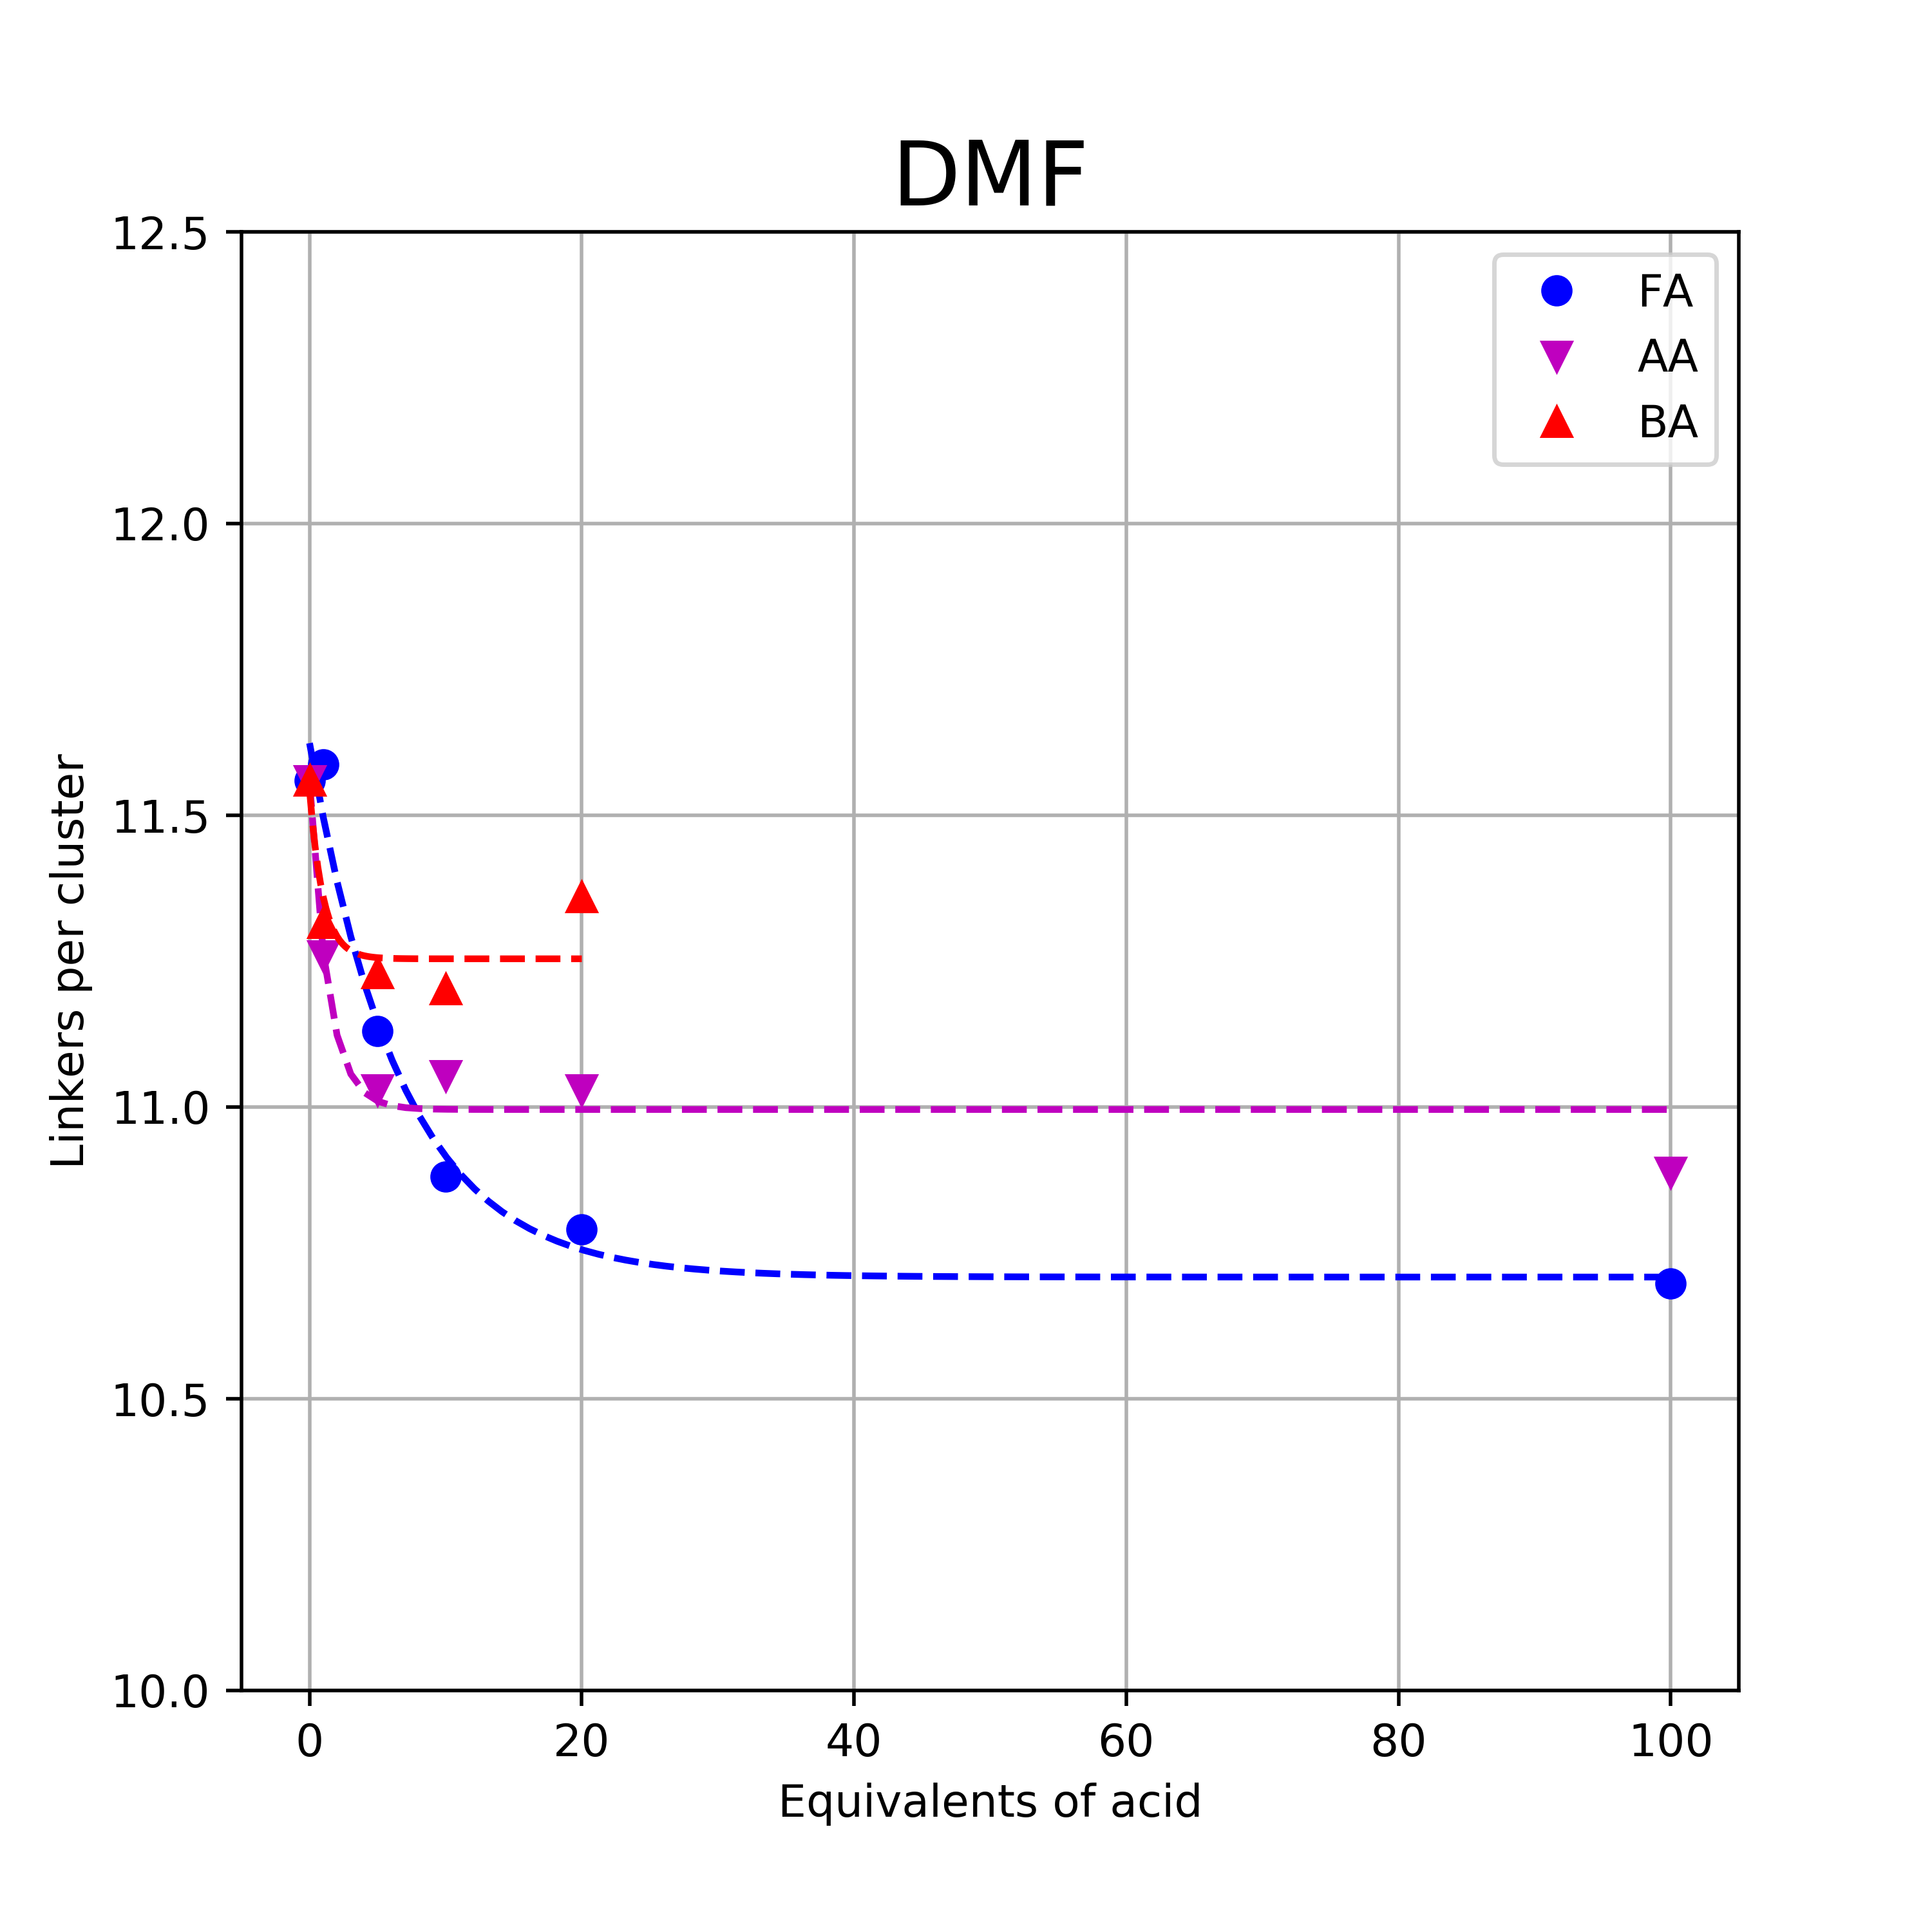
\includegraphics[width=\textwidth]{tga/DMF-def-overview}%
        \caption{}%
        \label{def:fgr:tga-dmf-linkers}
    \end{subfigure}%
    \begin{subfigure}{0.25\linewidth}
        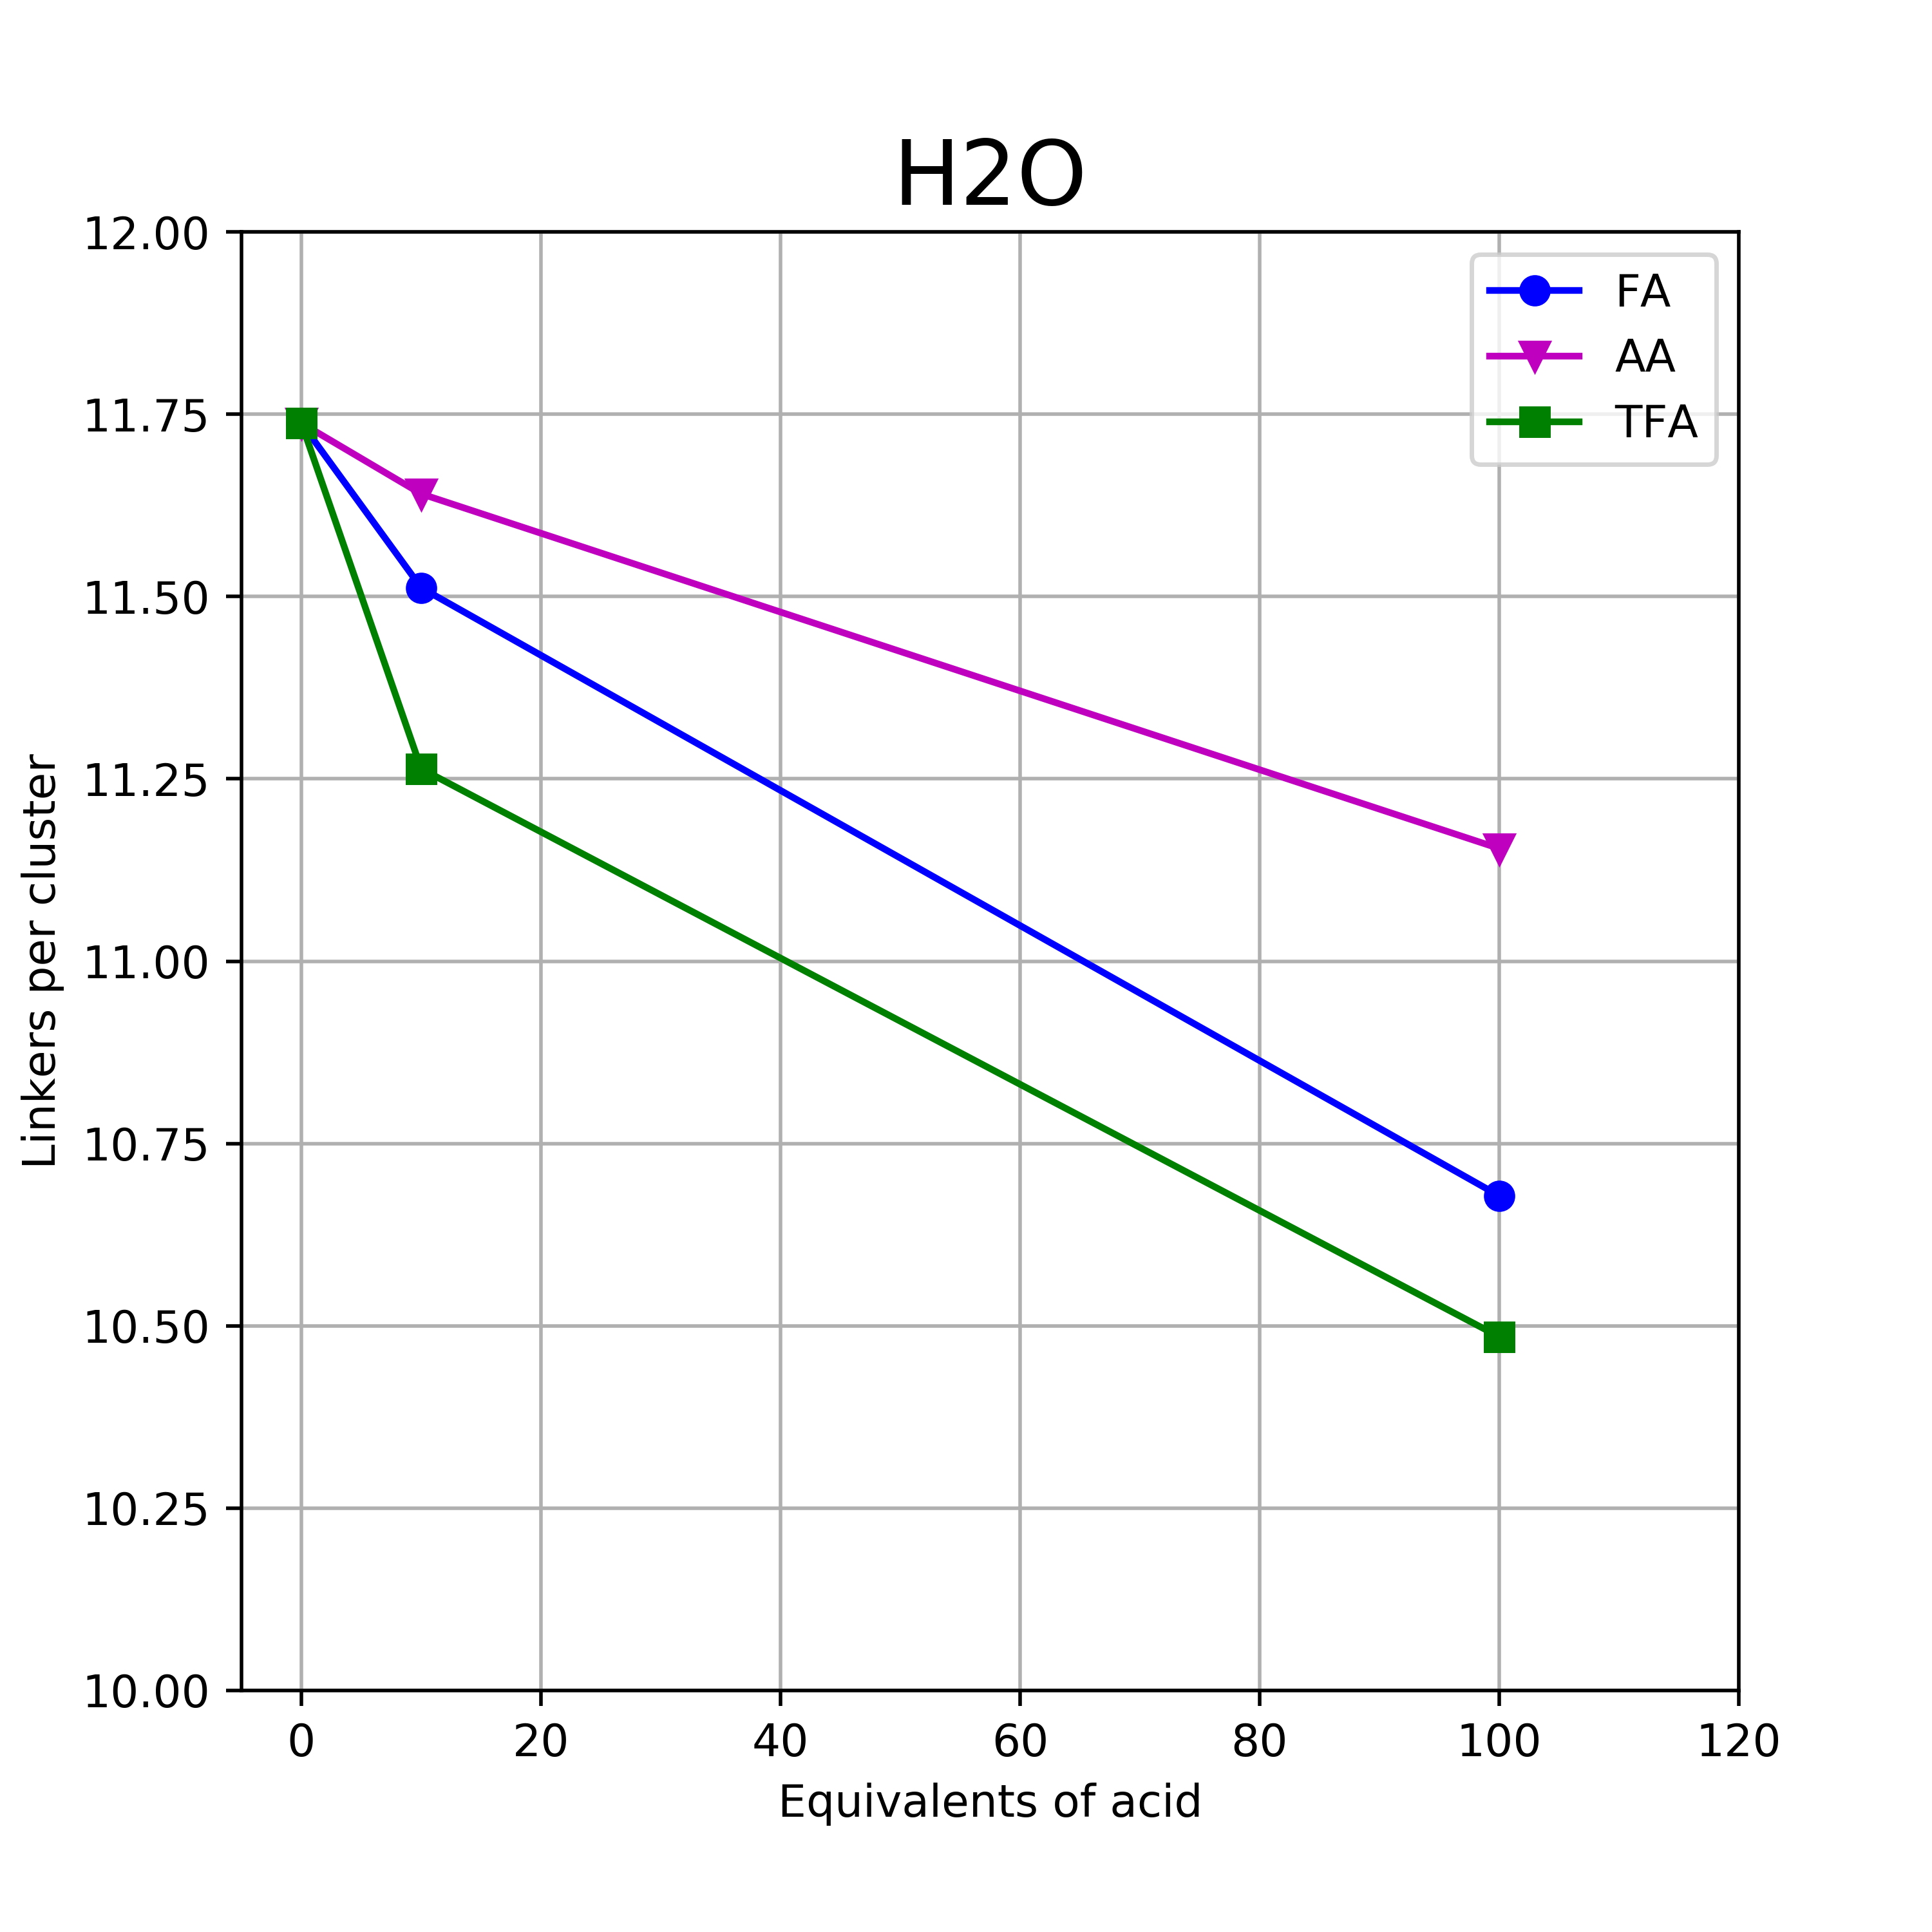
\includegraphics[width=\textwidth]{tga/H2O-def-overview}%
        \caption{}%
        \label{def:fgr:tga-h2o-linkers}
    \end{subfigure}%
    \begin{subfigure}{0.25\linewidth}
        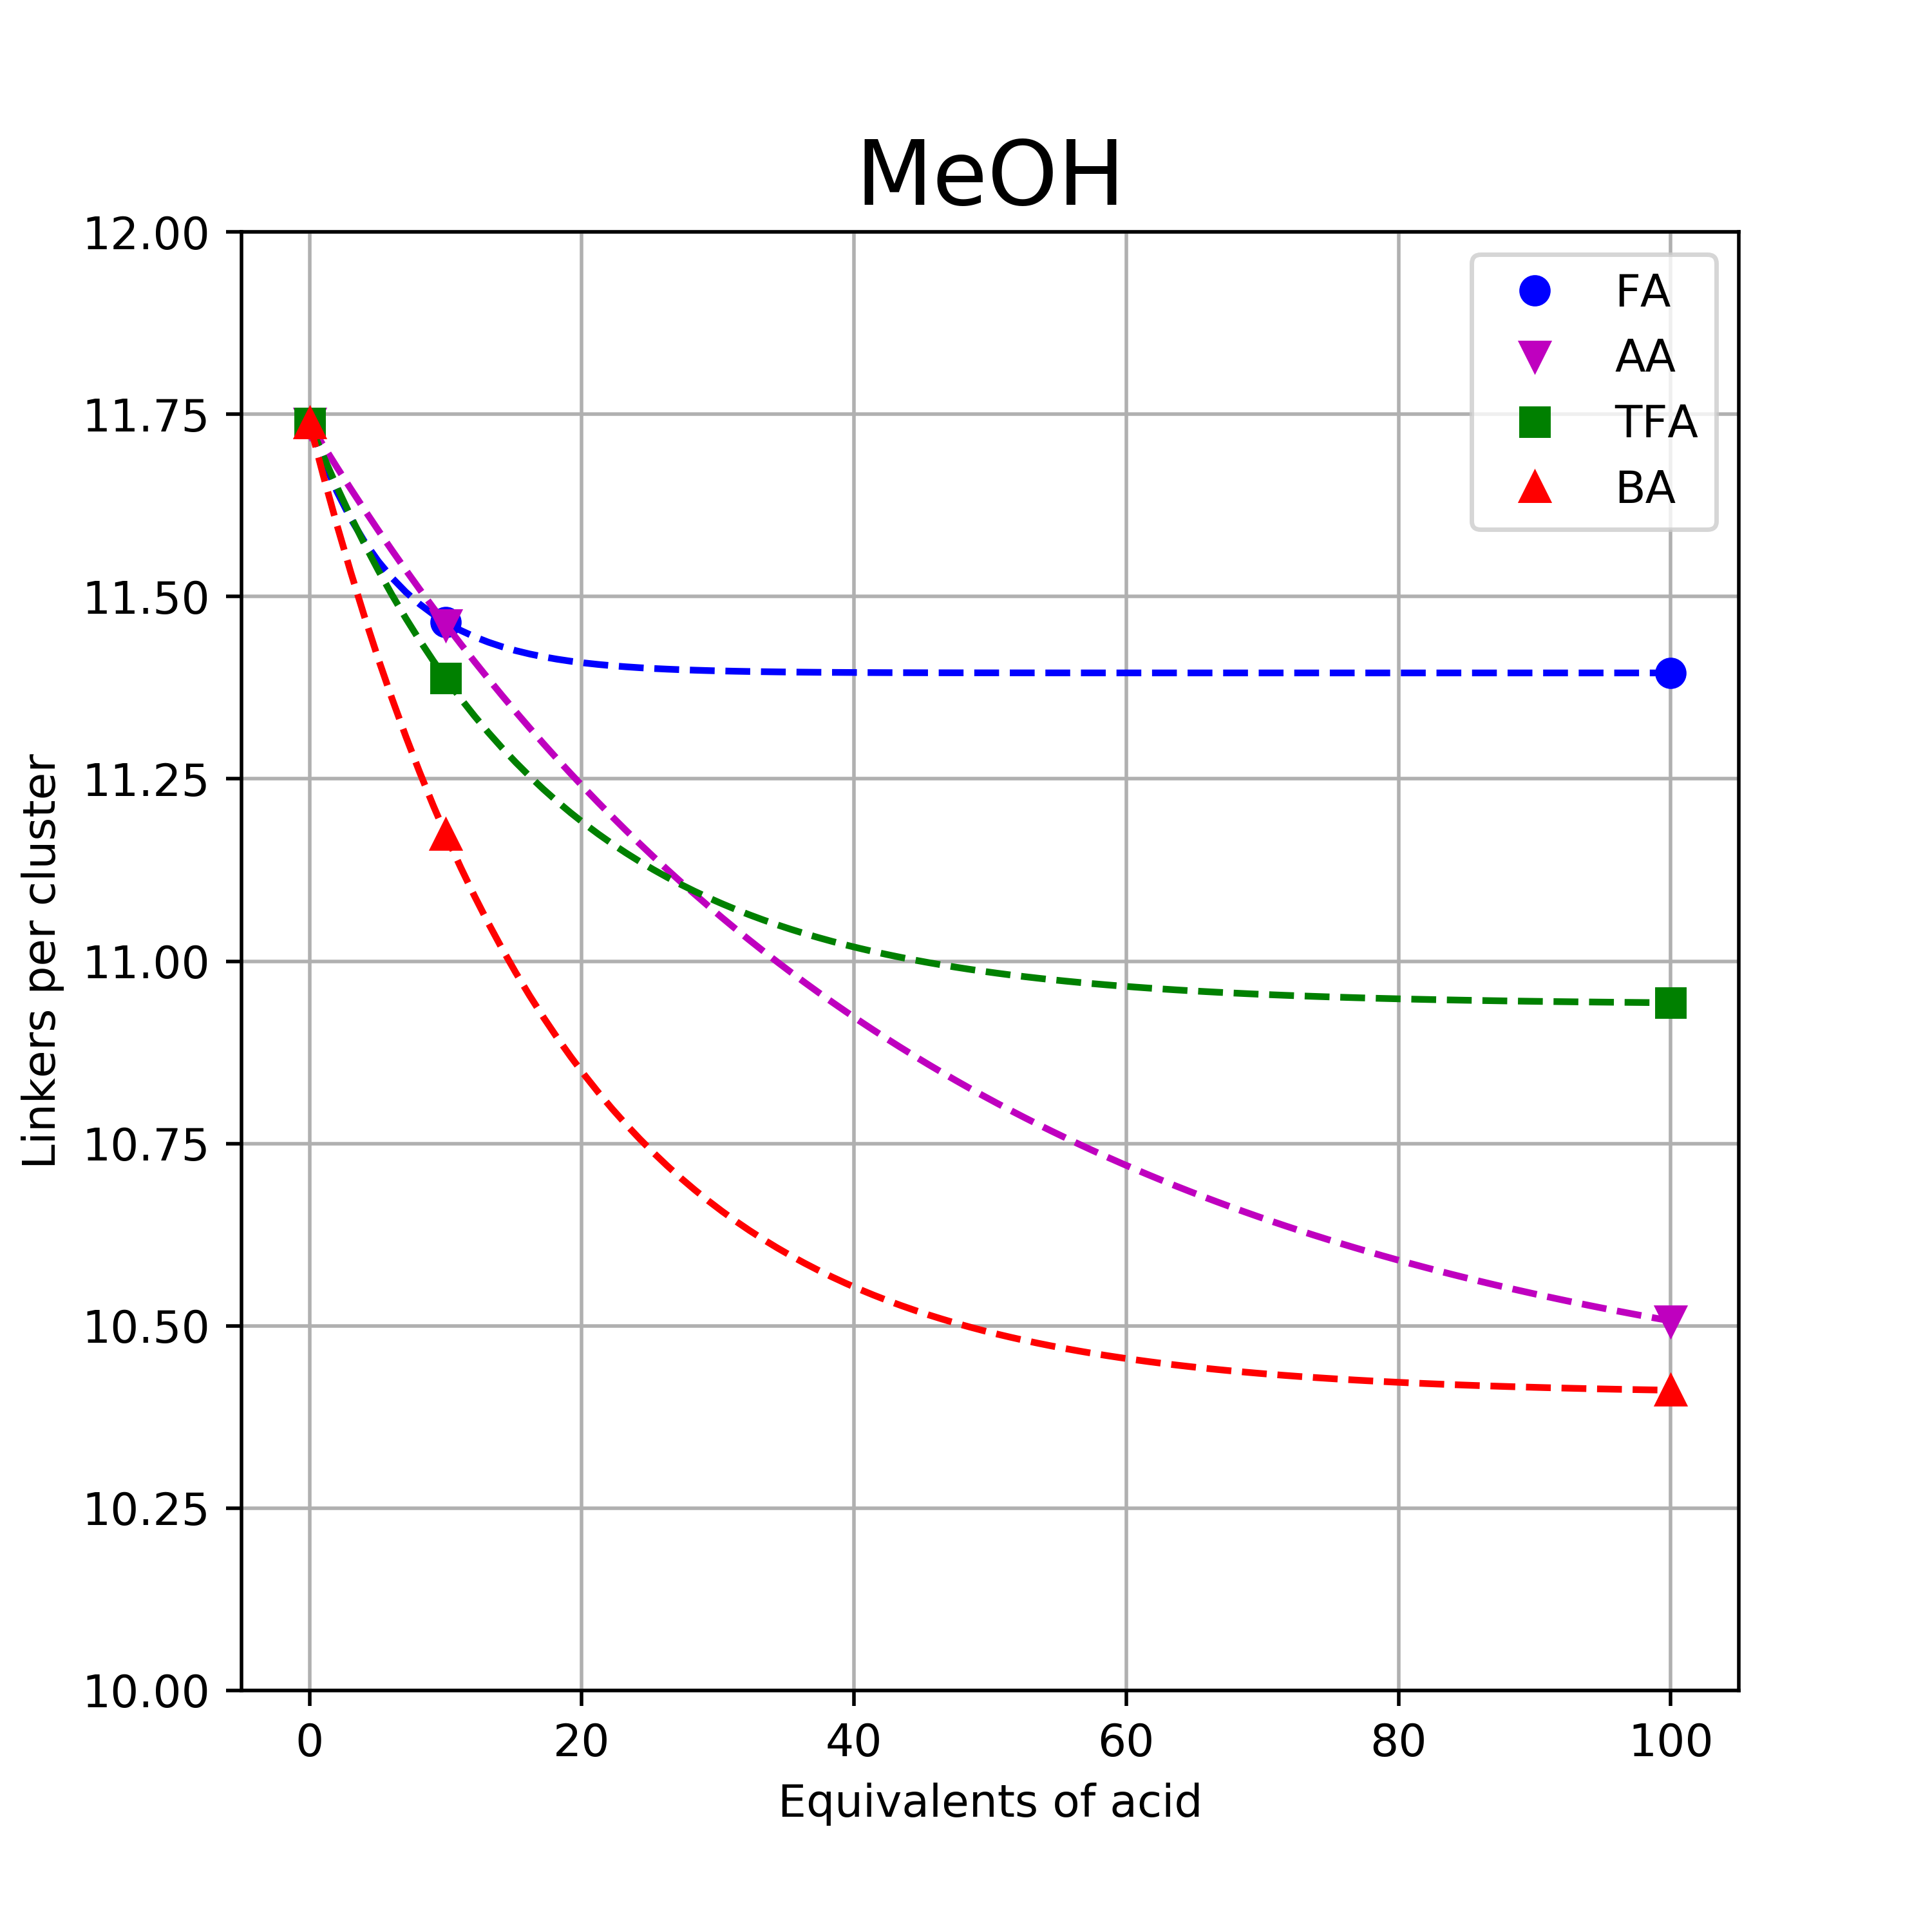
\includegraphics[width=\textwidth]{tga/MeOH-def-overview}%
        \caption{}%
        \label{def:fgr:tga-meoh-linkers}
    \end{subfigure}%
    \begin{subfigure}{0.25\linewidth}
        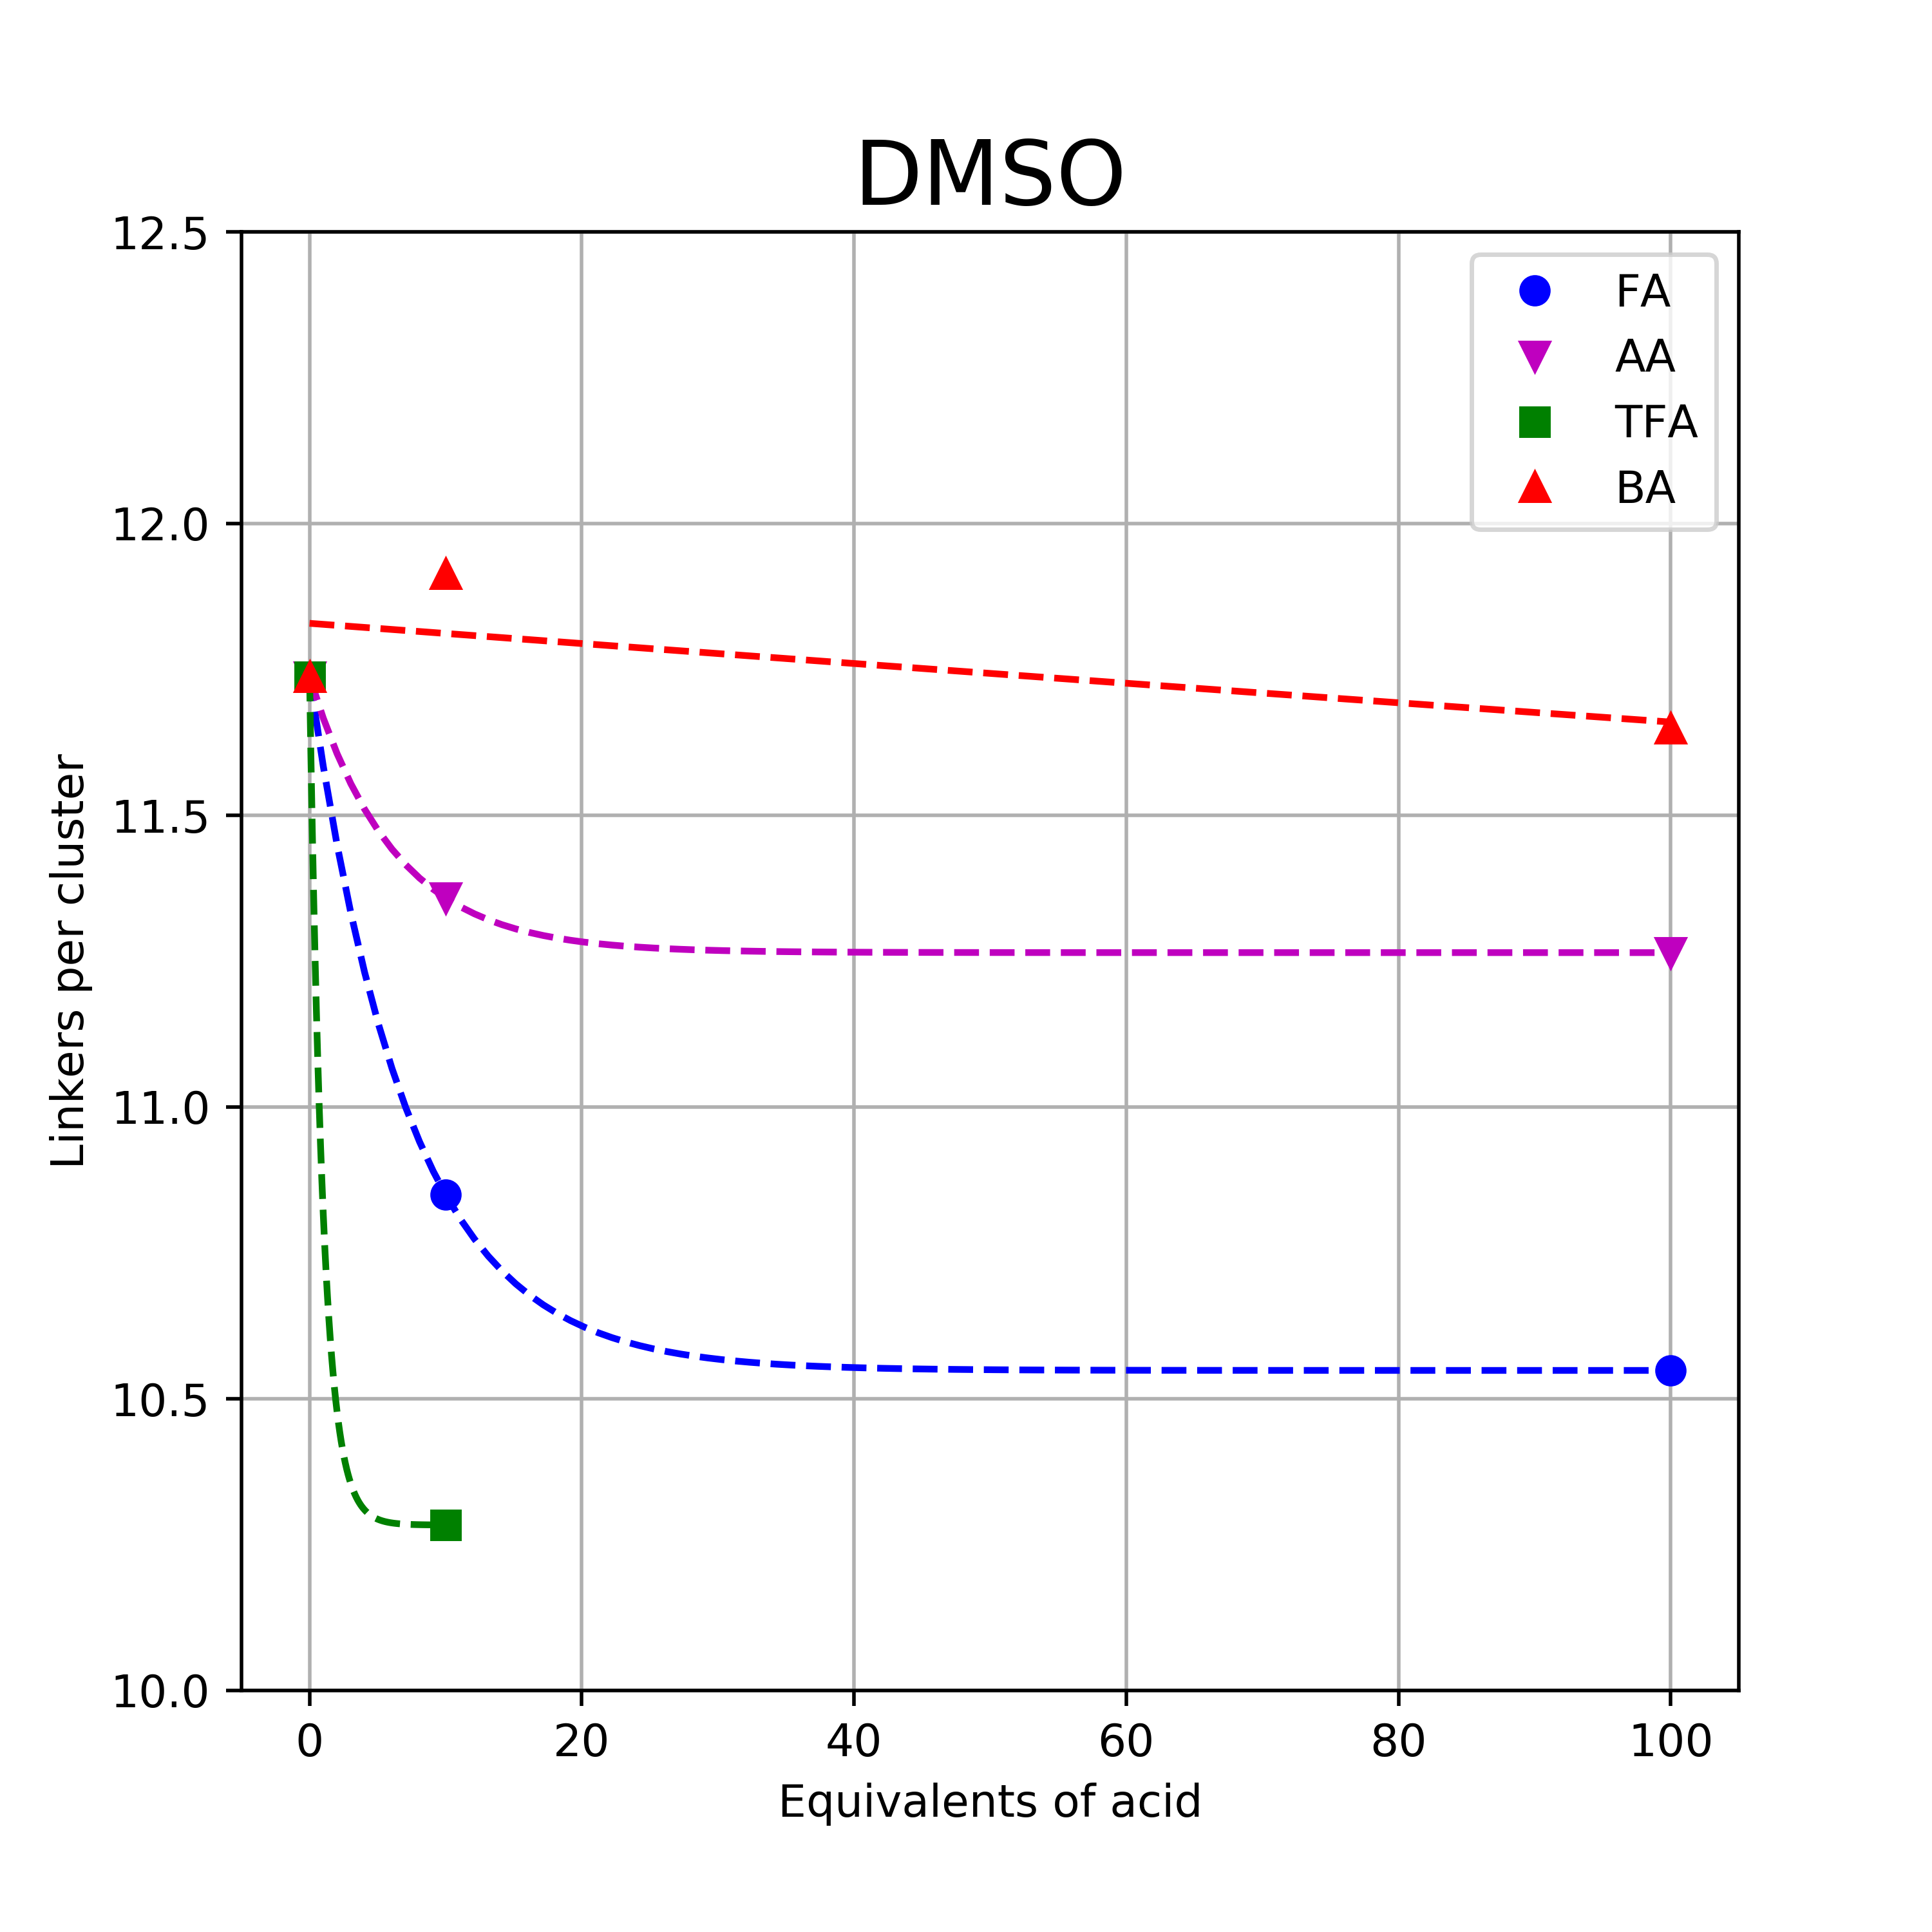
\includegraphics[width=\textwidth]{tga/DMSO-def-overview}%
        \caption{}%
        \label{def:fgr:tga-dmso-linkers}
    \end{subfigure}%

    \caption{Calculated linker-to-node ratio from the TGA curve 
    normalized mass at \SI{420}{\degreeCelsius} for (a) DMF 
    (b) \ce{H2O}, (c) \ce{MeOH} and (d) DMSO leached samples.
    A ratio of 12 to 1 corresponds to a completely defect-free
    structure. An exponential decay trendline is fitted to 
    each set of points.}%
    \label{def:fgr:tga-defects}
    
\end{figure}

For the nitrogen adsorption dataset, the predictors described in the 
previous section have been calculated using the pyGAPS framework
(\autoref{pyg}). The Henry constant is determined through the 
initial slope method, with a linear section found below 
\(10^{-4}~p/p_0\). Pore volume is taken as the liquid density
of the amount adsorbed at \(0.8~p/p_0\), assuming that the 
nitrogen is in a liquid-like state in the MOF pores. The pore
size distribution was calculated through the Horvatz-Kawazoe
method for micropores, the Dollimore-Heal method for mesopores
and DFT kernel fitting for a multiscale distribution. While 
the applicability of these methods for determination of absolute
pore size may be questioned, they can be readily used to
compare between different samples of the same material.
In general, the leaching process has a positive effect on 
both surface area and pore volume, both of which increase 
with a higher concentration of acid used. The strength of 
the initial interaction of the nitrogen probe with the pore 
walls is changed as well, with more defective samples likely
to have a more pronounced interaction, either through the introduction
of CUS or modification of pore environment.

\begin{figure}[htb]
    \centering

    \begin{subfigure}{0.25\linewidth}
        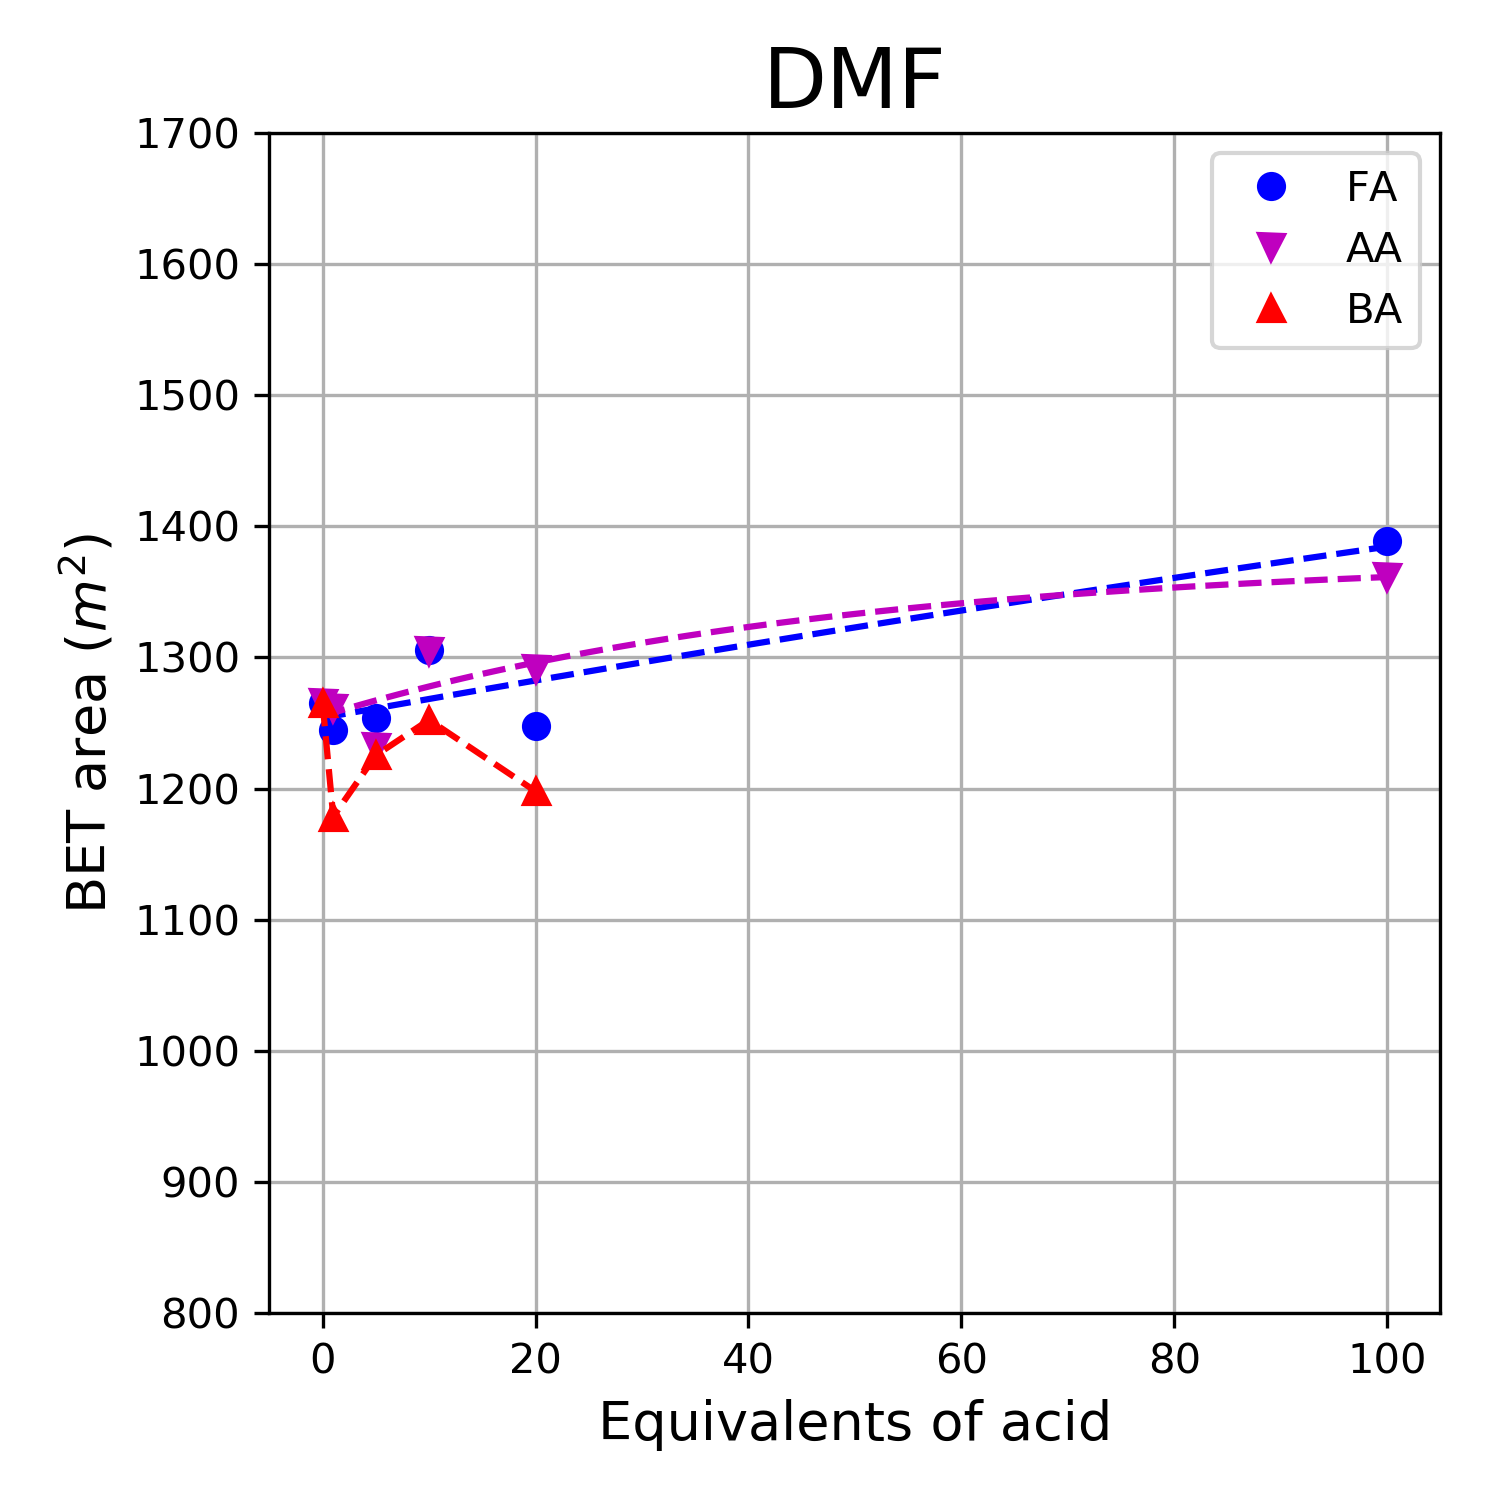
\includegraphics[width=\textwidth]{n2phys/dmf-area}%
        \caption{}%
        \label{def:fgr:n2phys-dmf-area}
    \end{subfigure}%
    \begin{subfigure}{0.25\linewidth}
        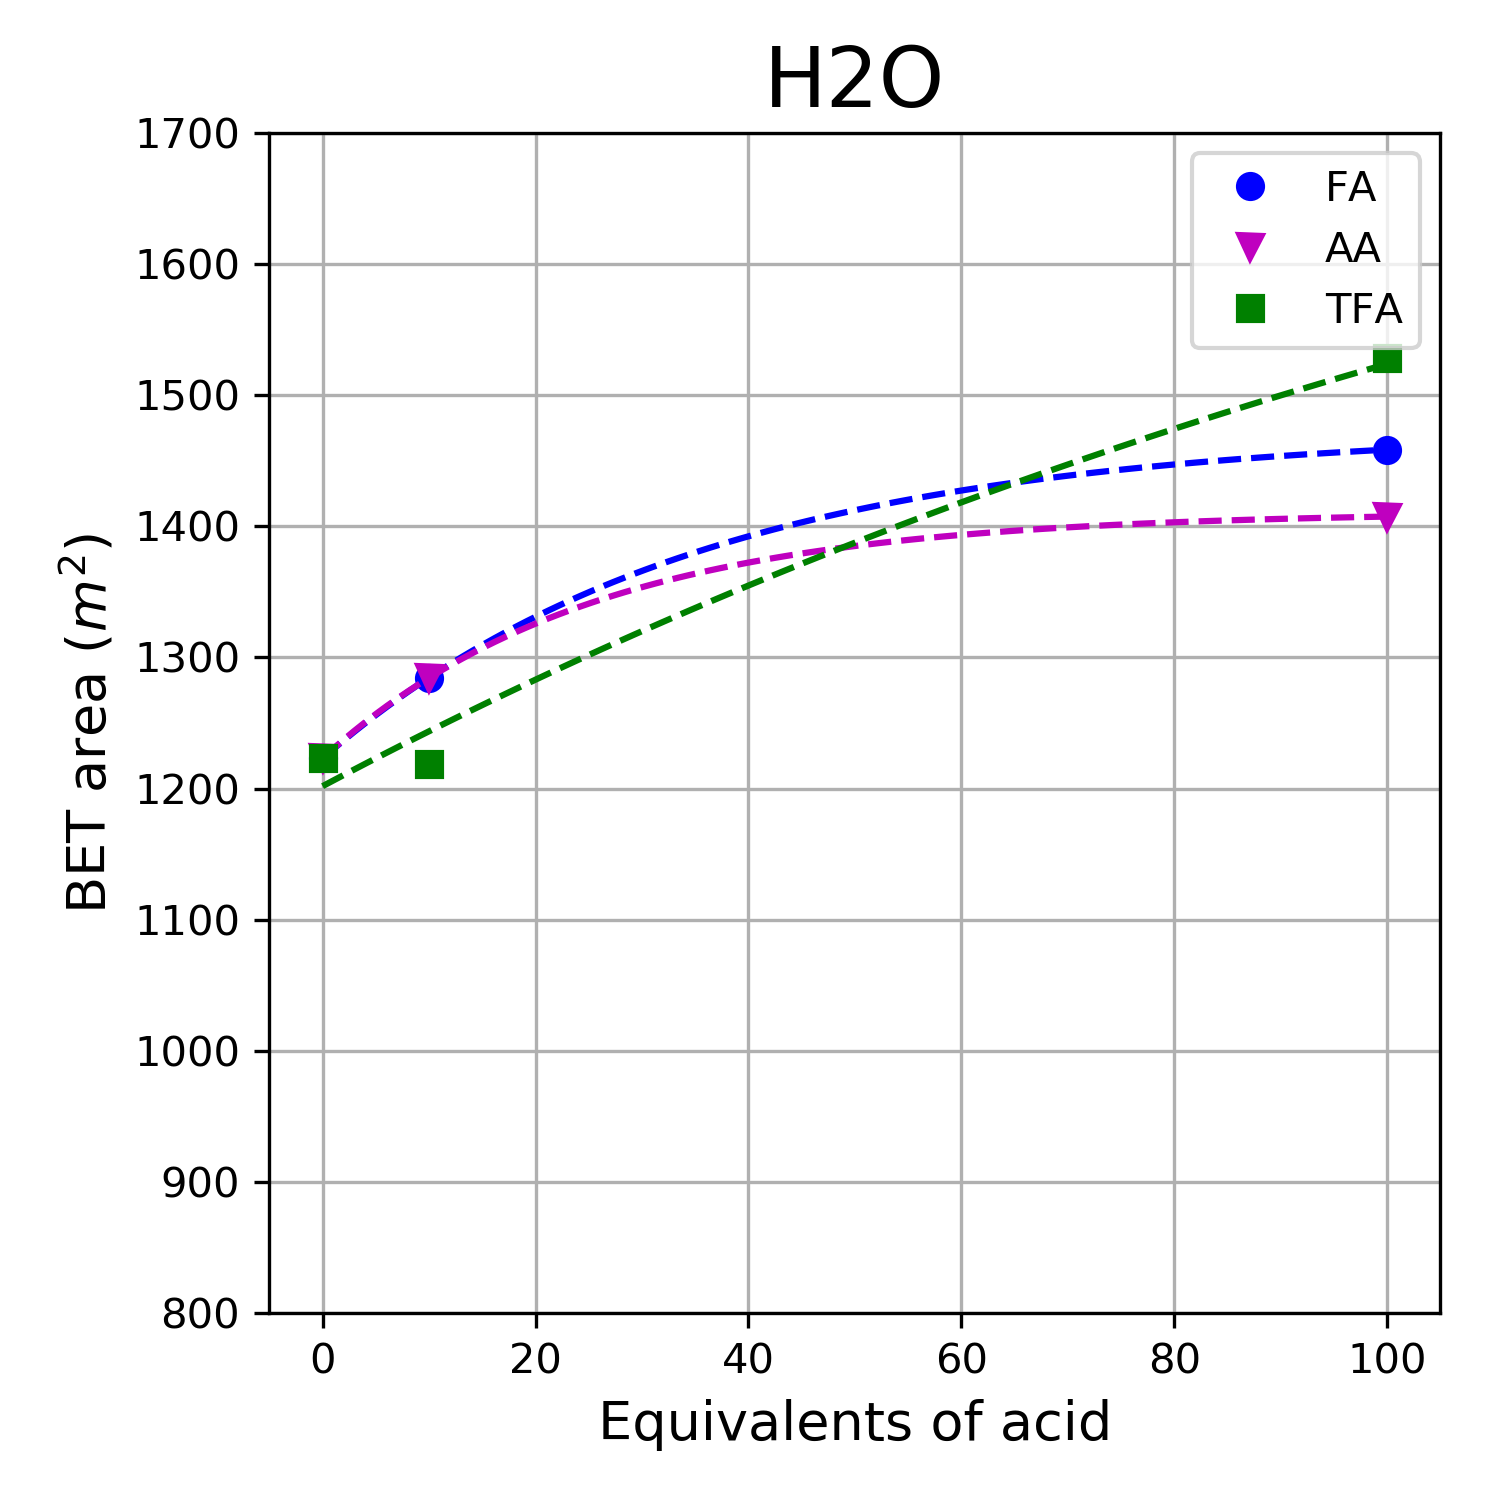
\includegraphics[width=\textwidth]{n2phys/h2o-area}%
        \caption{}%
        \label{def:fgr:n2phys-h2o-area}
    \end{subfigure}%
    \begin{subfigure}{0.25\linewidth}
        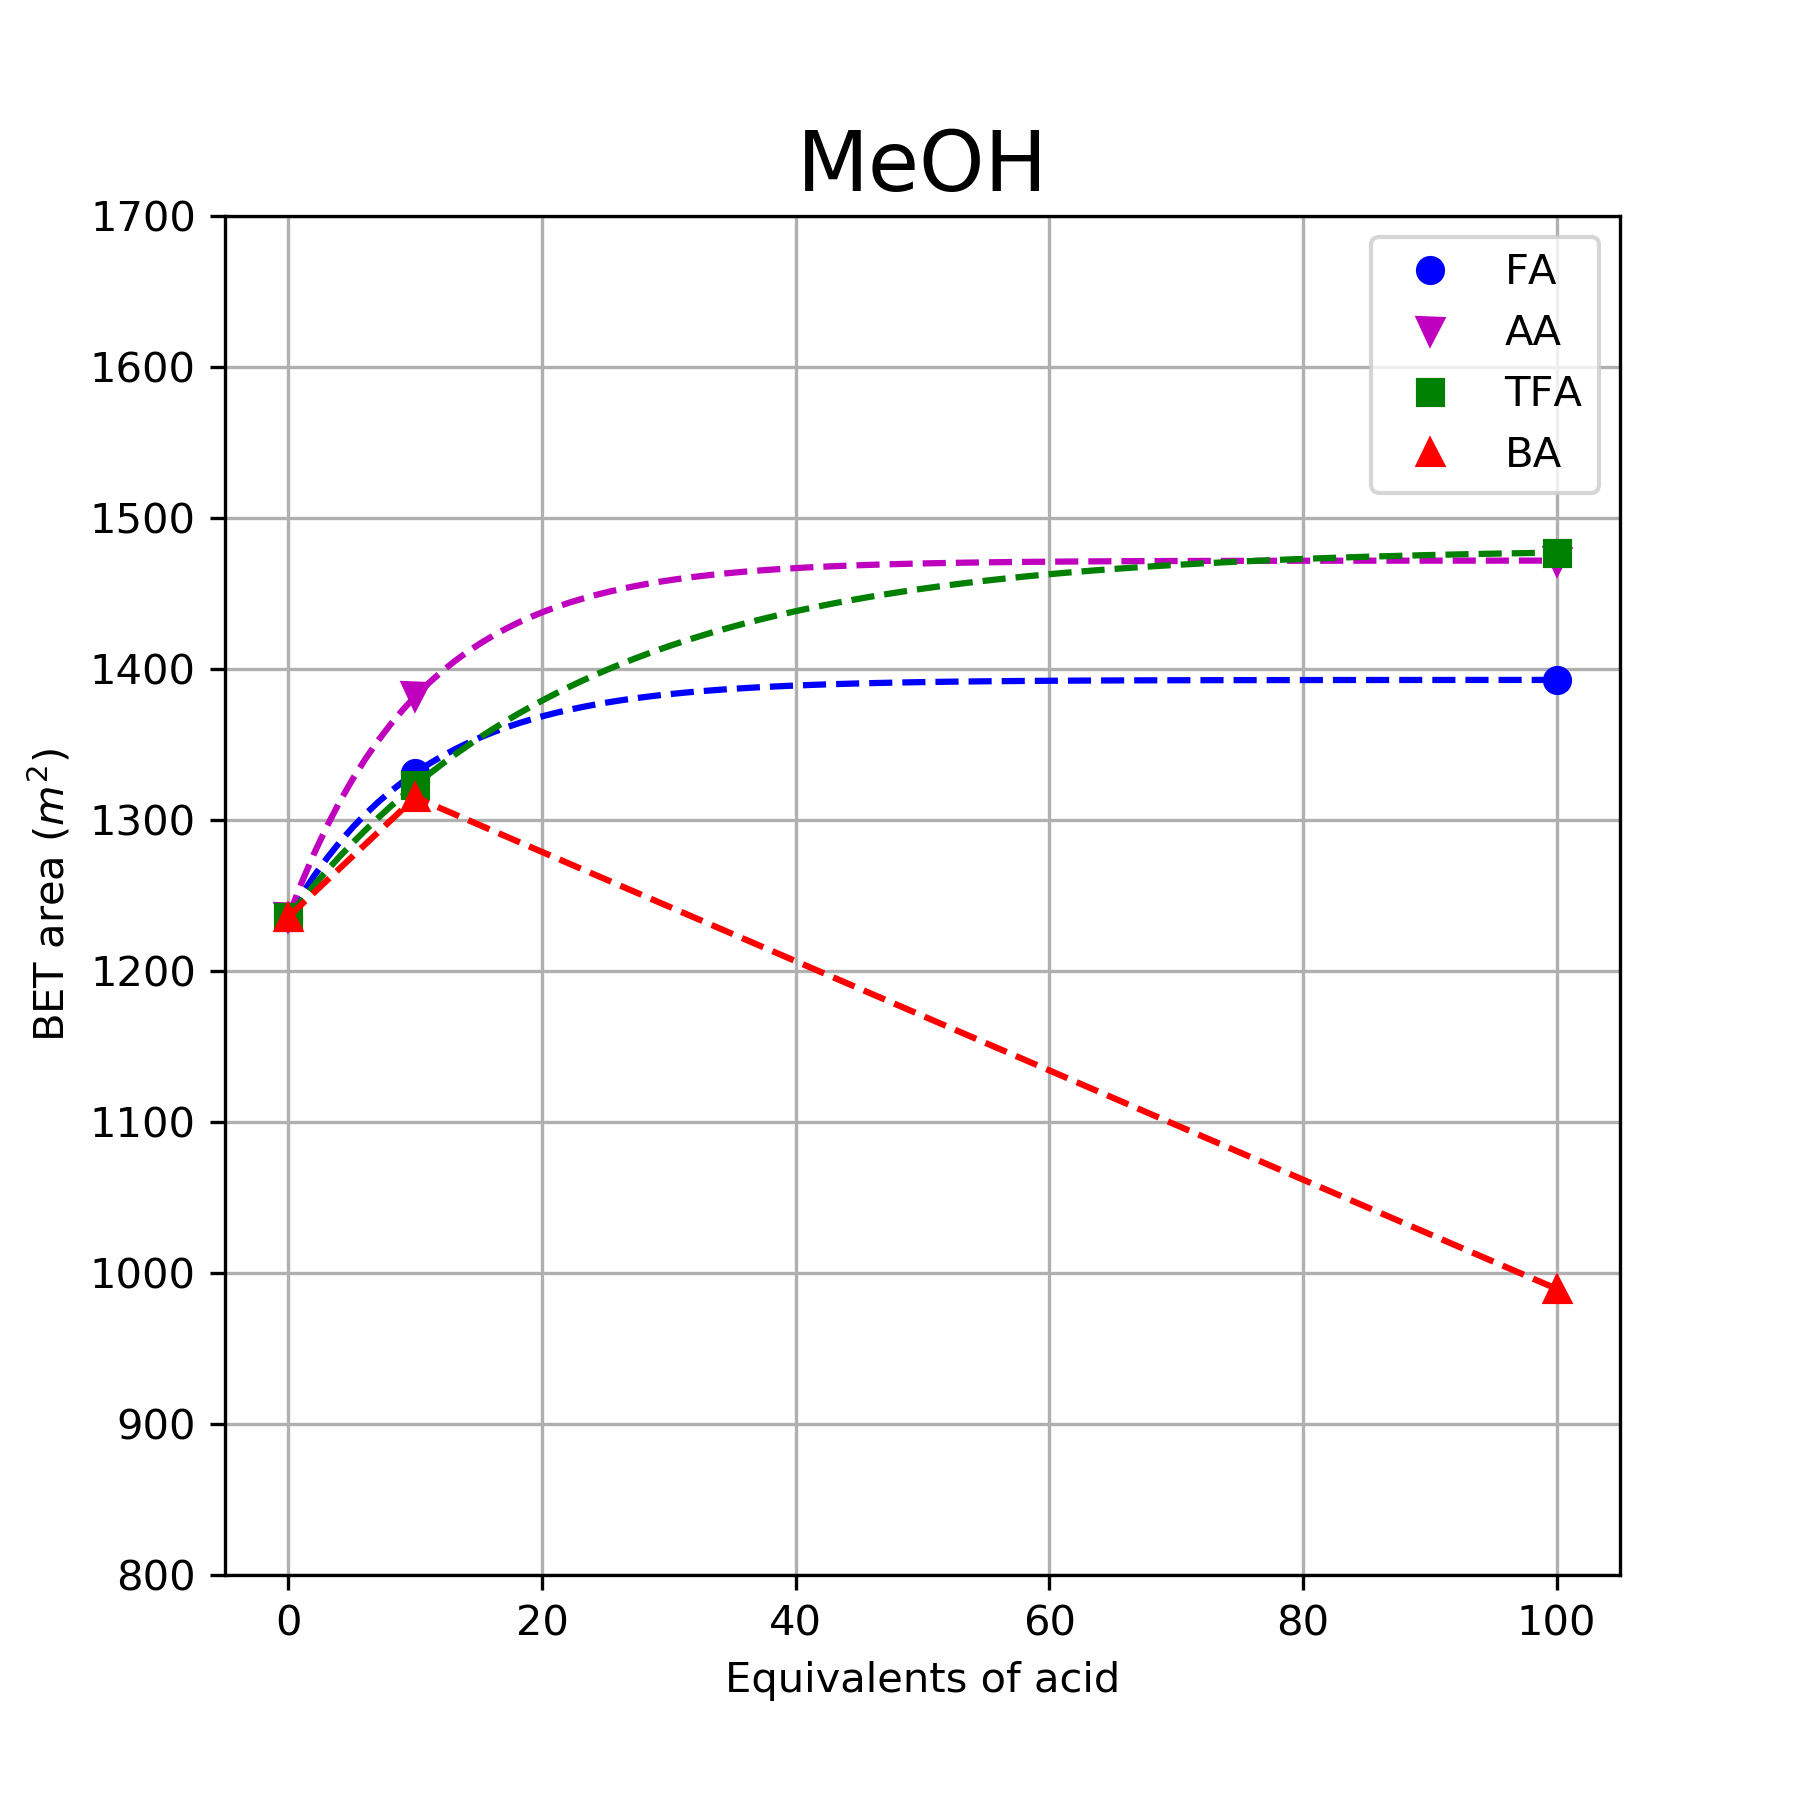
\includegraphics[width=\textwidth]{n2phys/meoh-area}%
        \caption{}%
        \label{def:fgr:n2phys-meoh-area}
    \end{subfigure}%
    \begin{subfigure}{0.25\linewidth}
        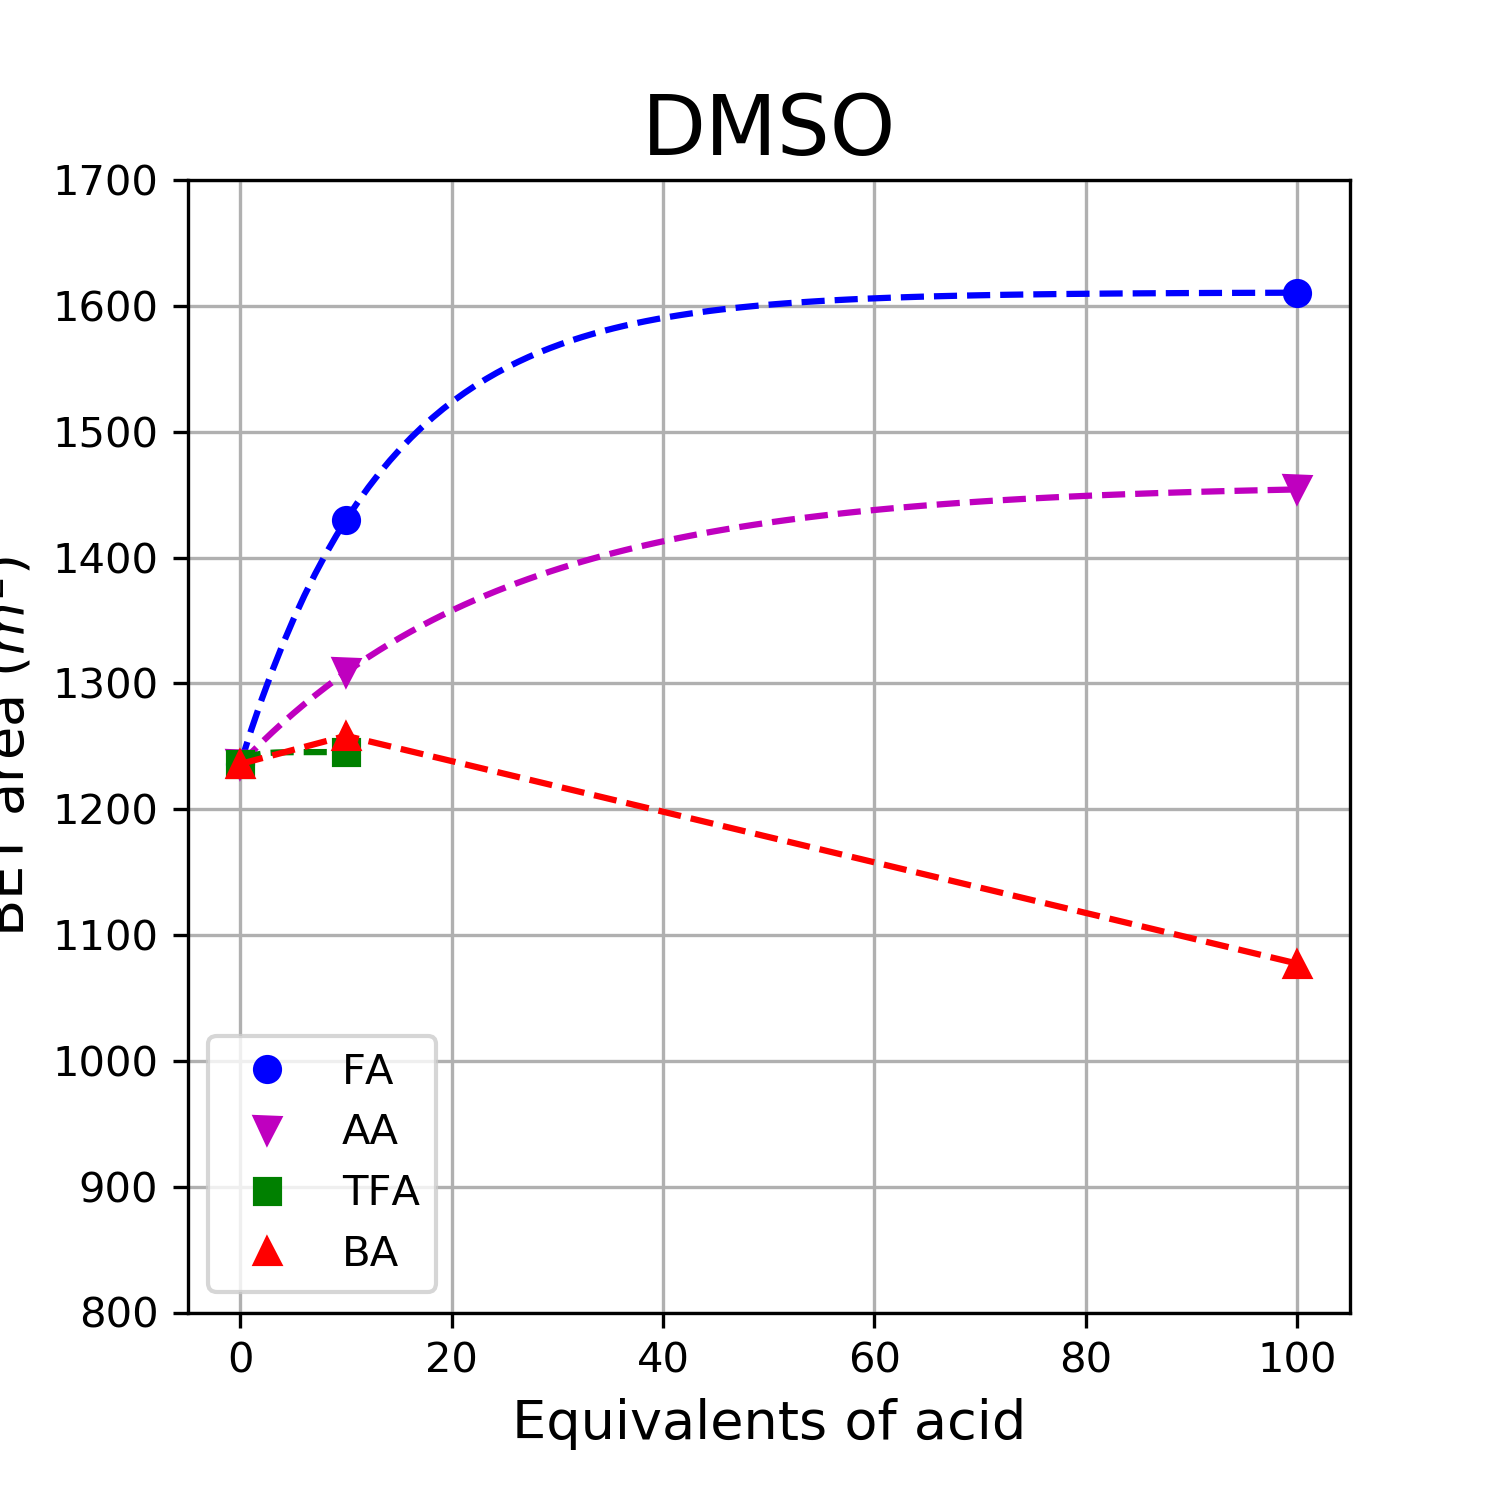
\includegraphics[width=\textwidth]{n2phys/dmso-area}%
        \caption{}%
        \label{def:fgr:n2phys-dmso-area}
    \end{subfigure}%

    \begin{subfigure}{0.25\linewidth}
        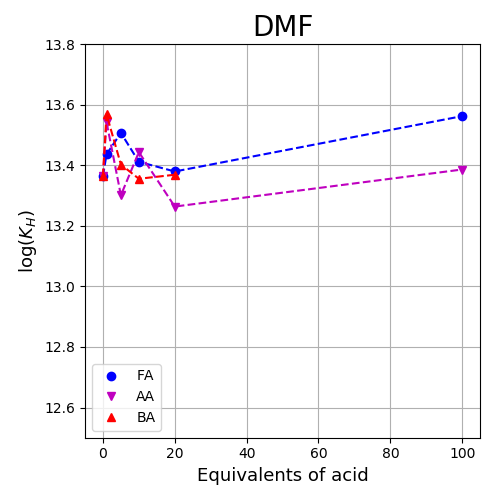
\includegraphics[width=\textwidth]{n2phys/dmf-henry}%
        \caption{}%
        \label{def:fgr:n2phys-dmf-henry}
    \end{subfigure}%
    \begin{subfigure}{0.25\linewidth}
        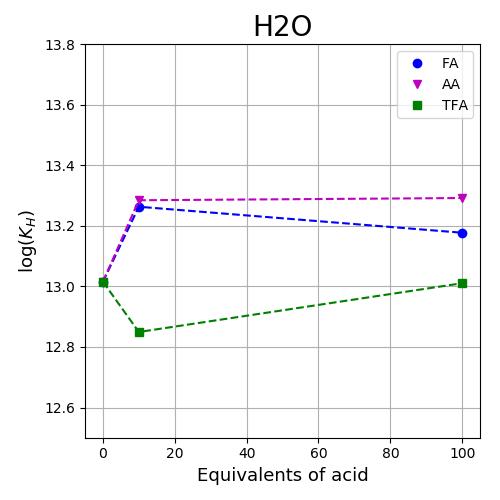
\includegraphics[width=\textwidth]{n2phys/h2o-henry}%
        \caption{}%
        \label{def:fgr:n2phys-h2o-henry}
    \end{subfigure}%
    \begin{subfigure}{0.25\linewidth}
        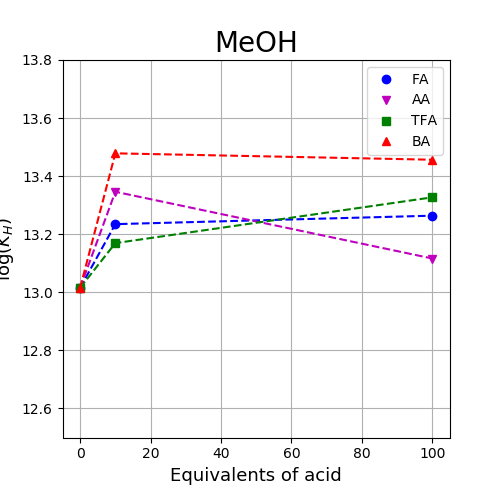
\includegraphics[width=\textwidth]{n2phys/meoh-henry}%
        \caption{}%
        \label{def:fgr:n2phys-meoh-henry}
    \end{subfigure}%
    \begin{subfigure}{0.25\linewidth}
        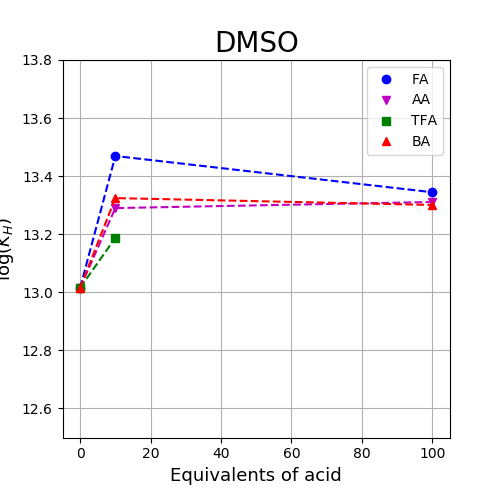
\includegraphics[width=\textwidth]{n2phys/dmso-henry}%
        \caption{}%
        \label{def:fgr:n2phys-dmso-henry}
    \end{subfigure}%

    \begin{subfigure}{0.25\linewidth}
        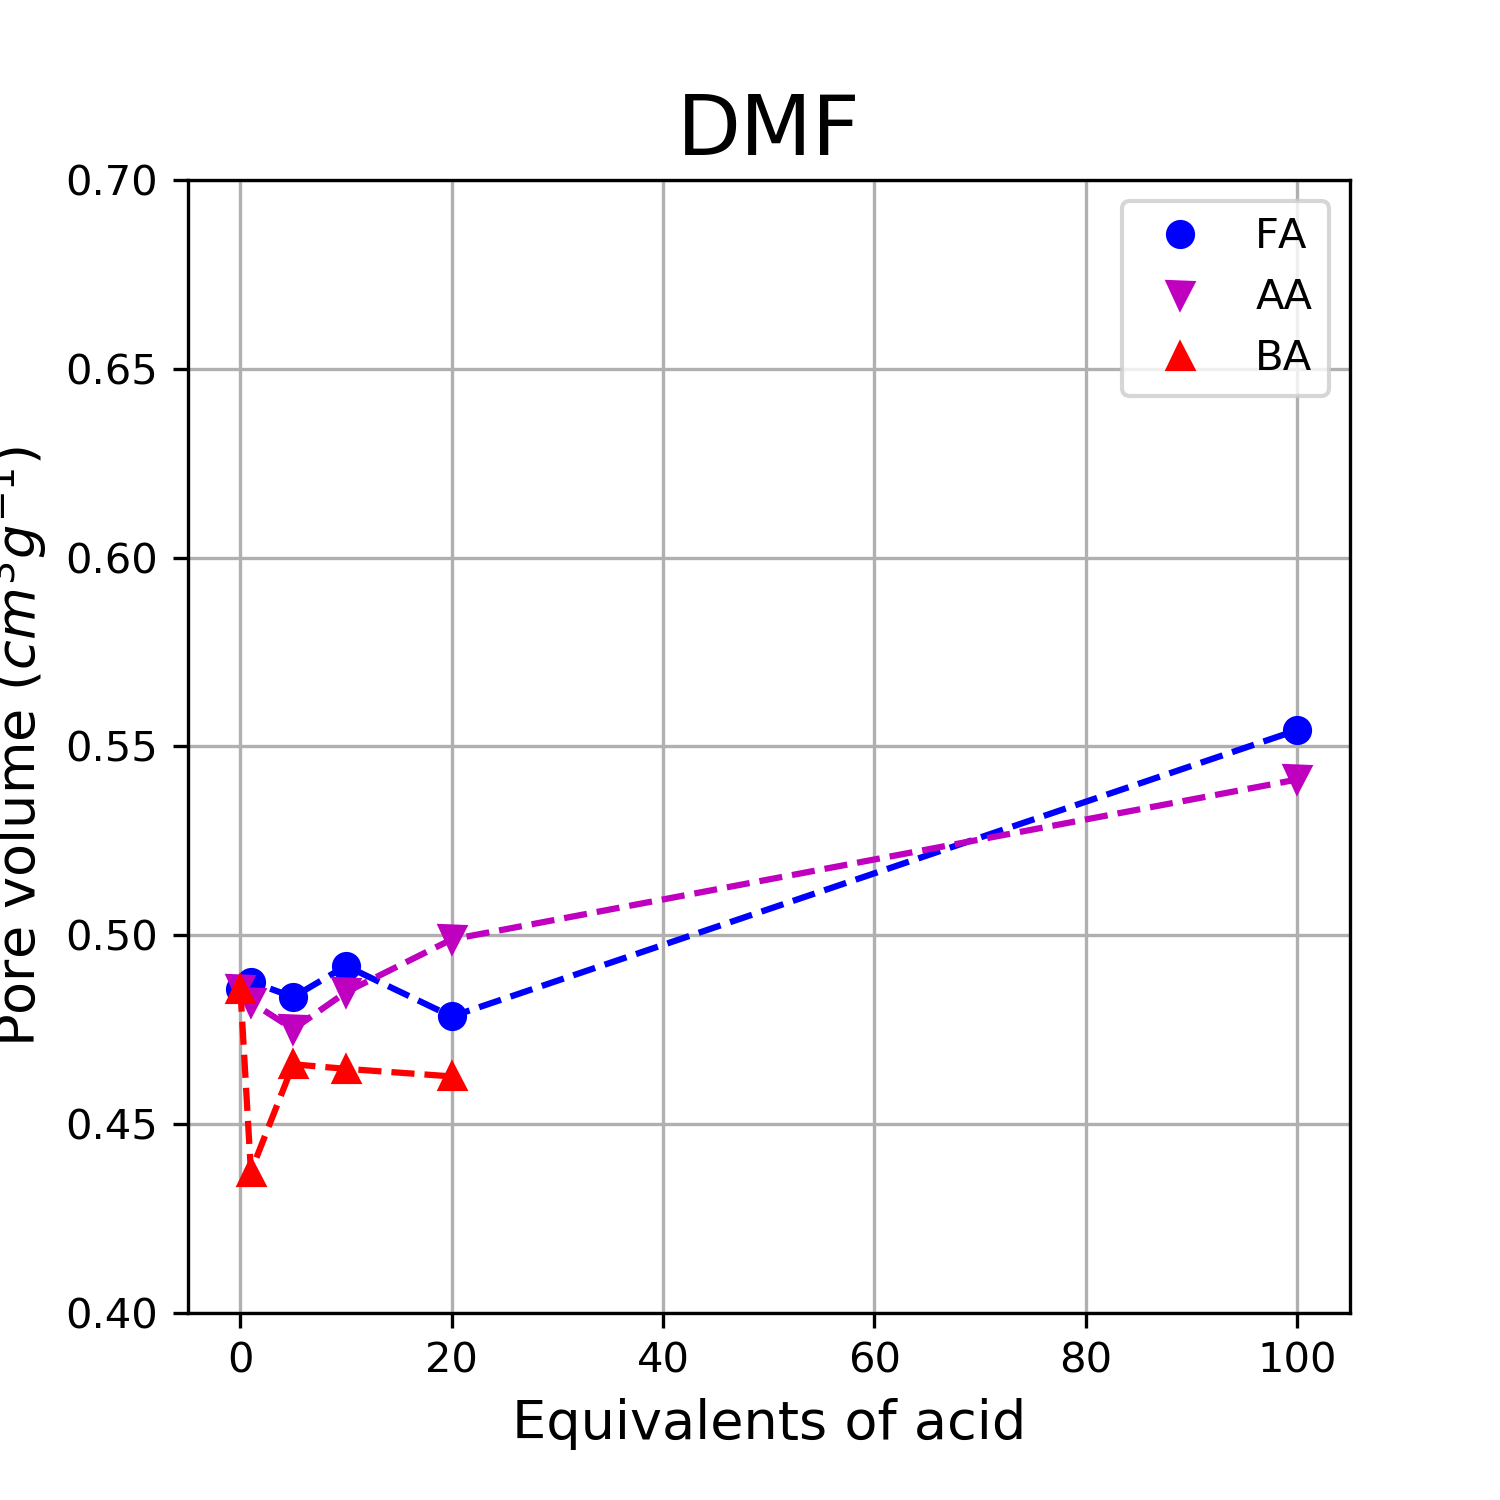
\includegraphics[width=\textwidth]{n2phys/dmf-porevol}%
        \caption{}%
        \label{def:fgr:n2phys-dmf-porevol}
    \end{subfigure}%
    \begin{subfigure}{0.25\linewidth}
        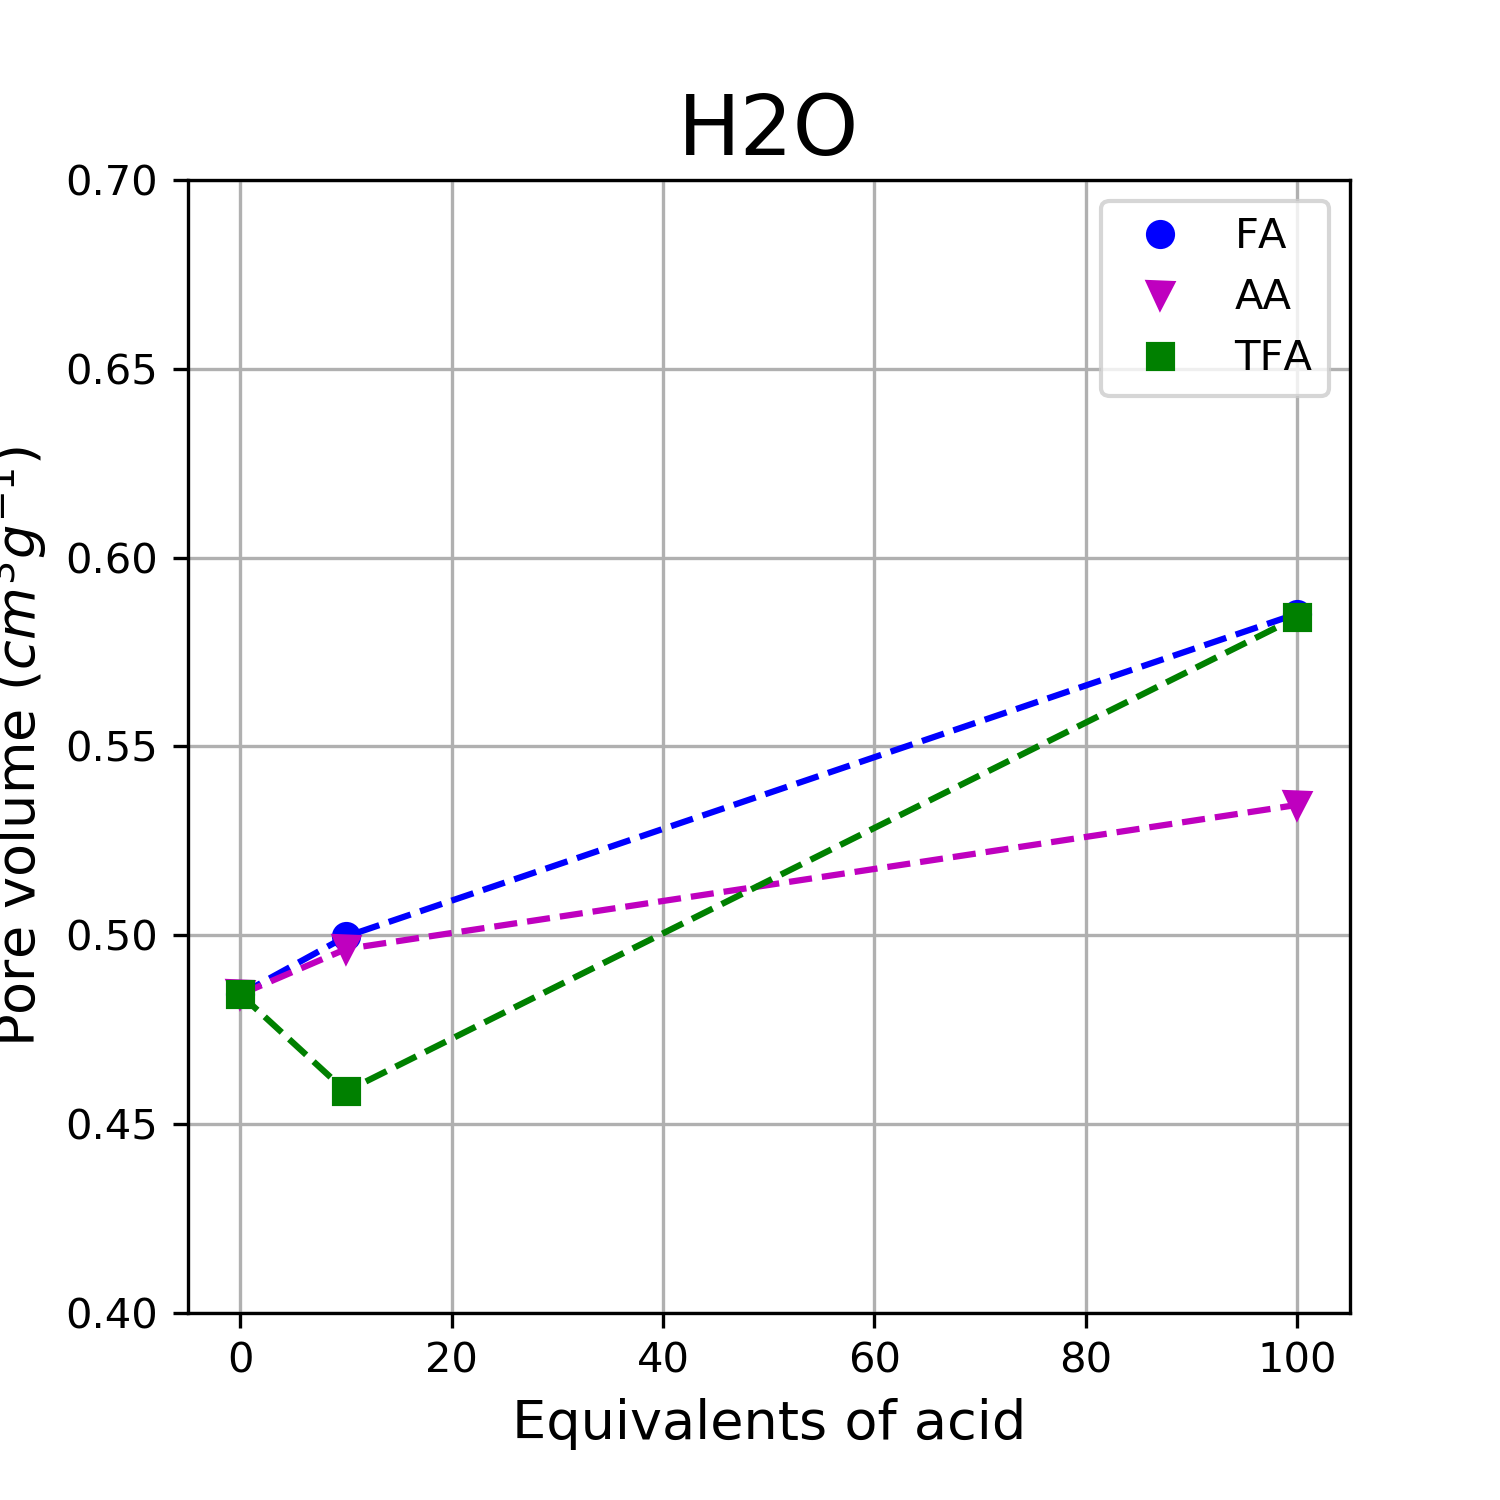
\includegraphics[width=\textwidth]{n2phys/h2o-porevol}%
        \caption{}%
        \label{def:fgr:n2phys-h2o-porevol}
    \end{subfigure}%
    \begin{subfigure}{0.25\linewidth}
        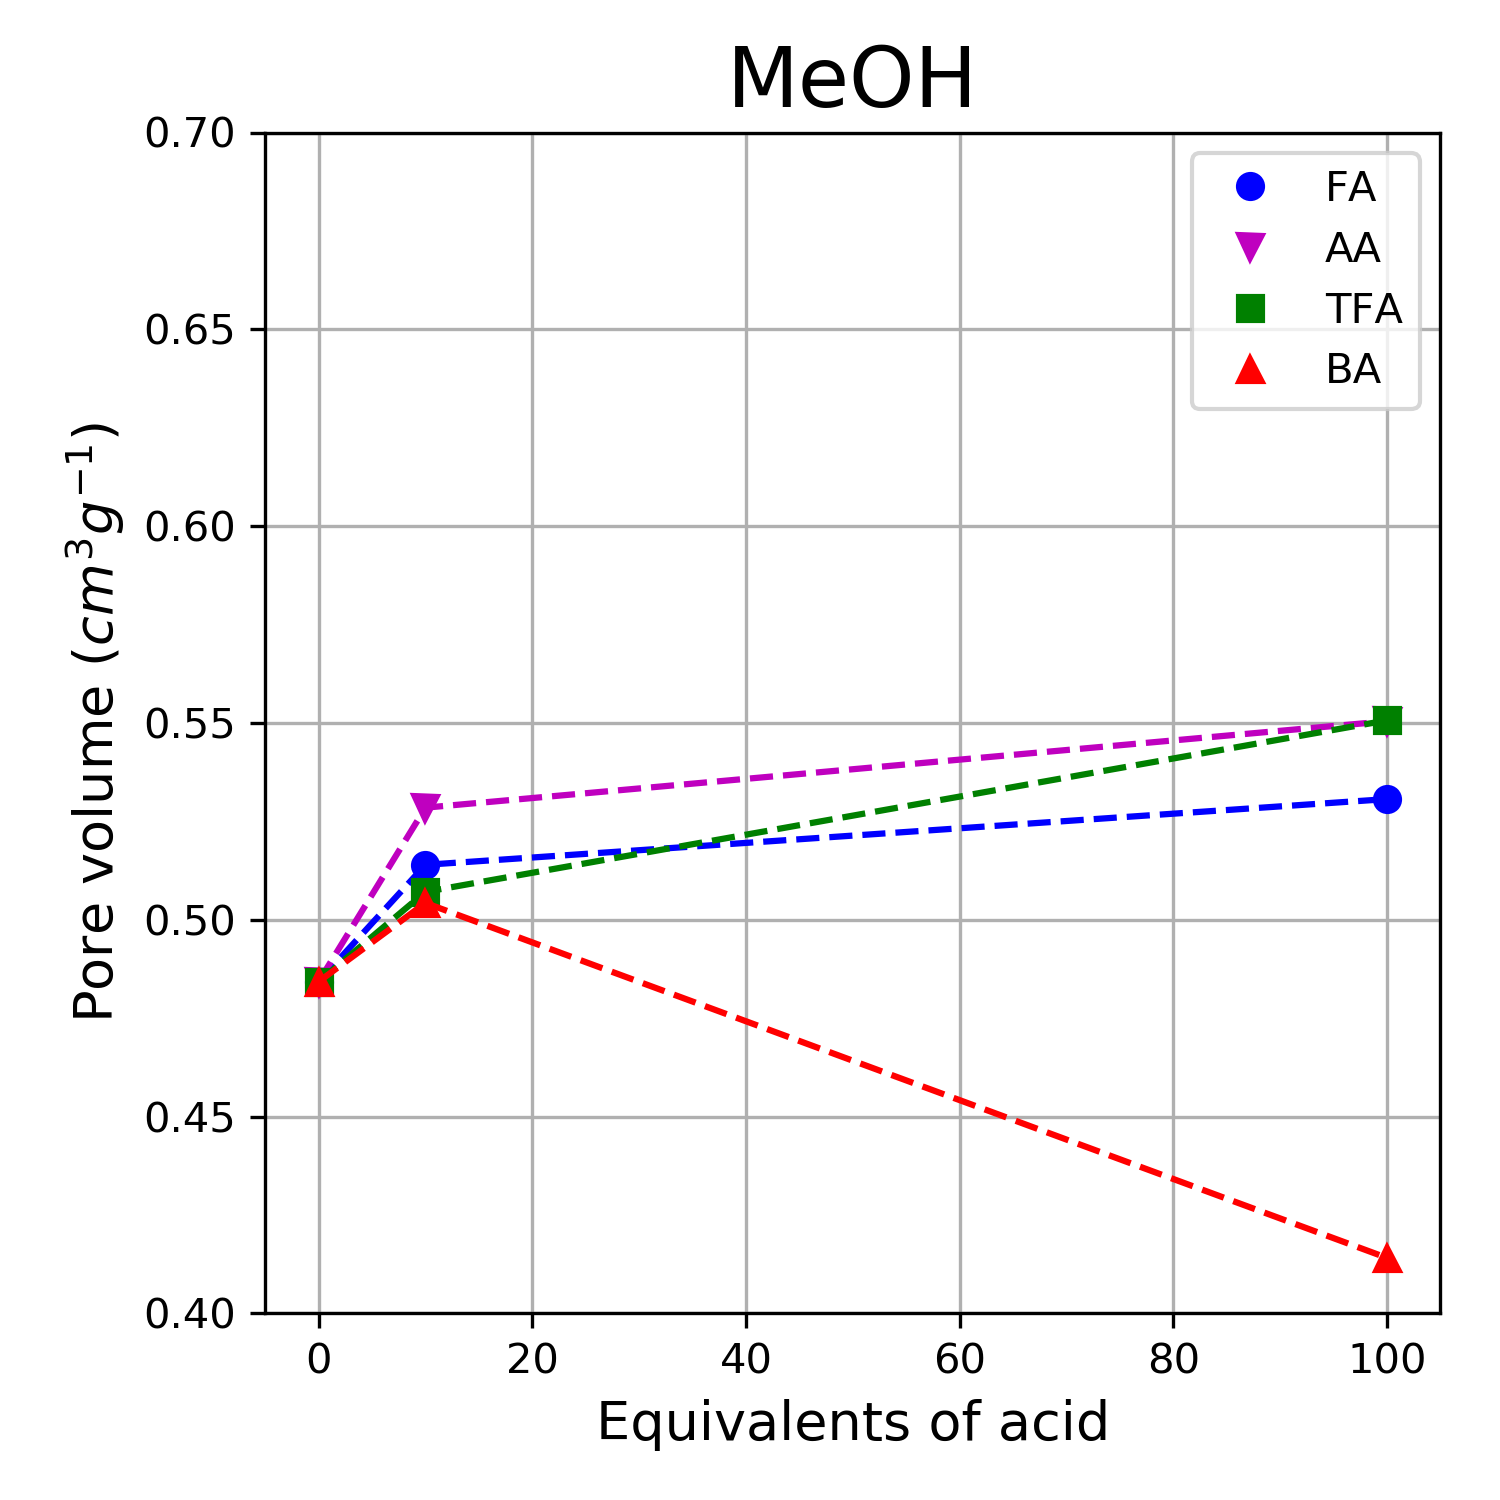
\includegraphics[width=\textwidth]{n2phys/meoh-porevol}%
        \caption{}%
        \label{def:fgr:n2phys-meoh-porevol}
    \end{subfigure}%
    \begin{subfigure}{0.25\linewidth}
        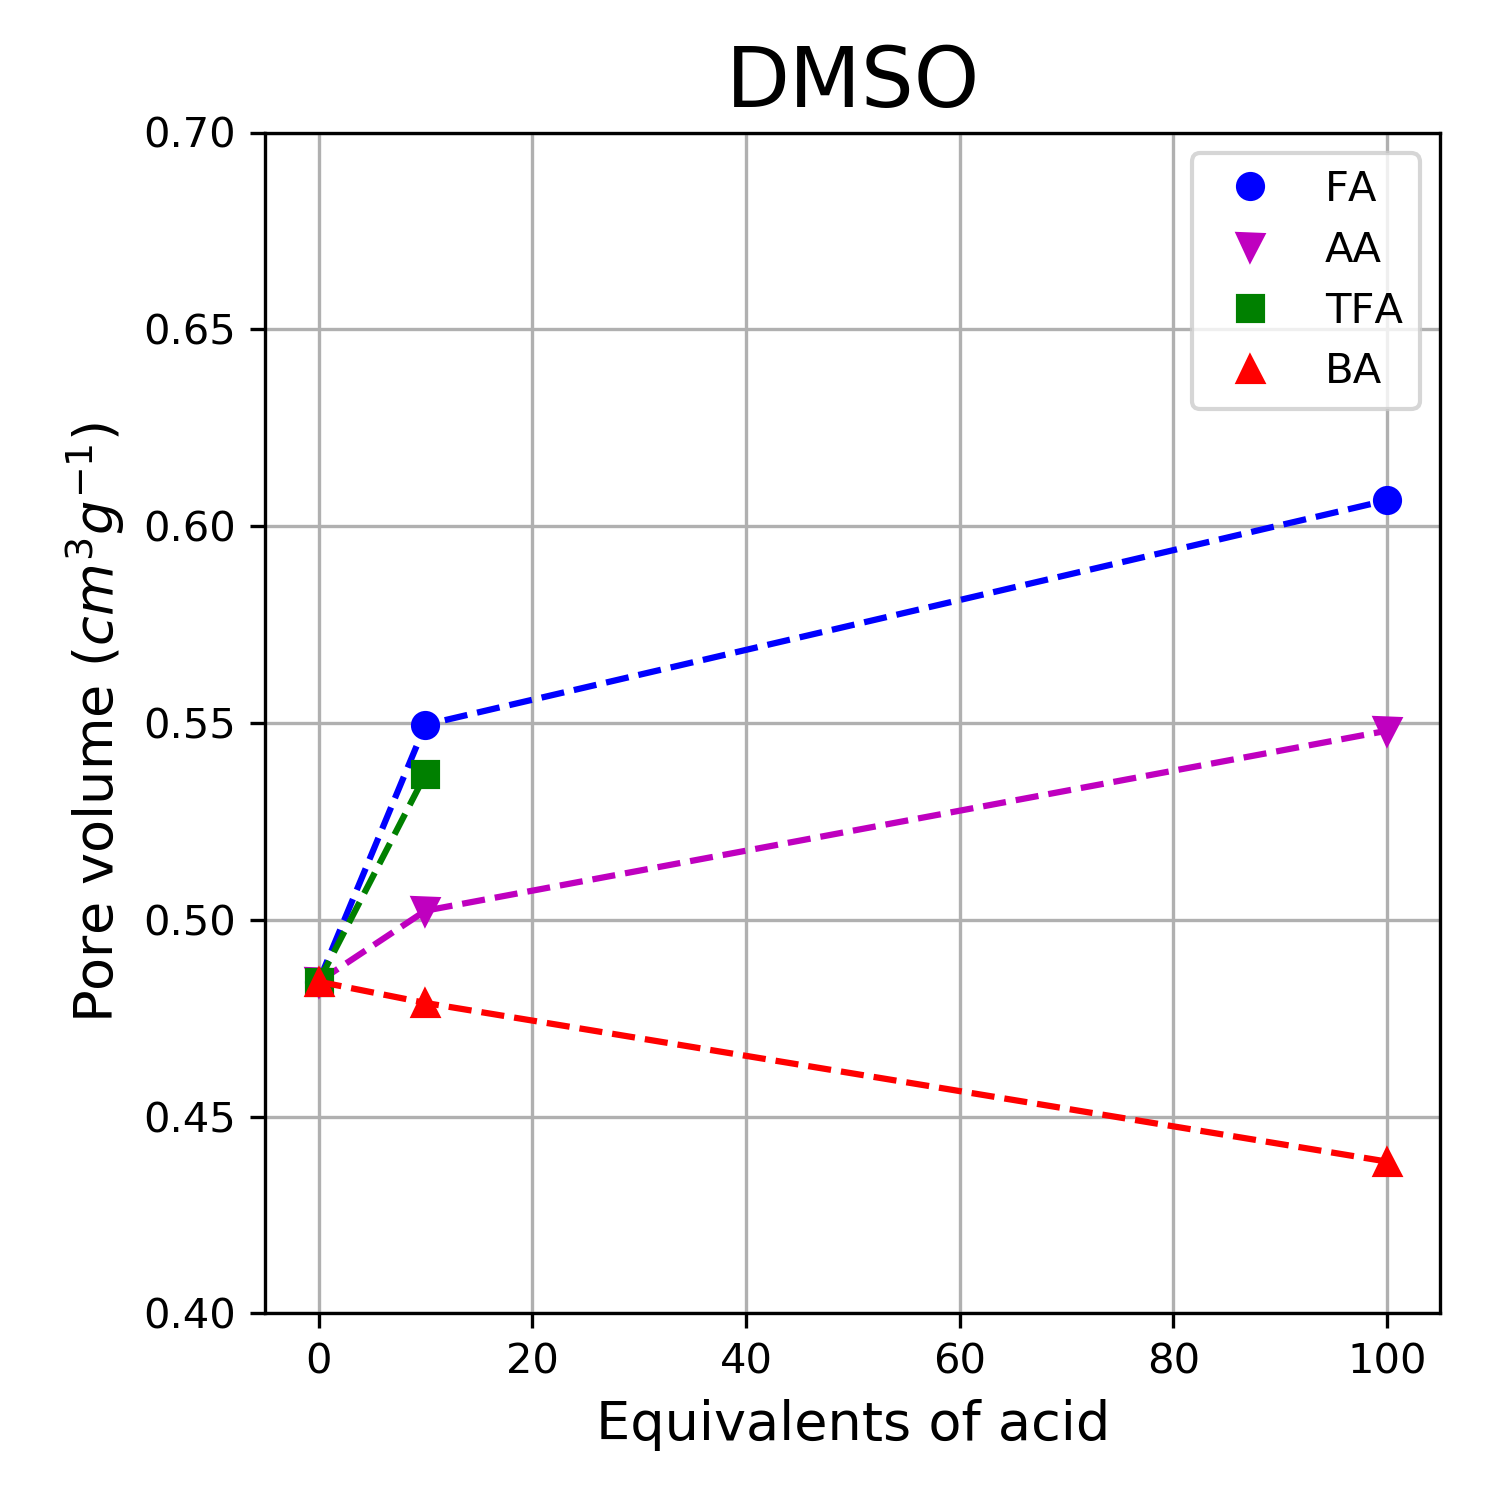
\includegraphics[width=\textwidth]{n2phys/dmso-porevol}%
        \caption{}%
        \label{def:fgr:n2phys-dmso-porevol}
    \end{subfigure}%

    \caption{Characterisation of all samples through predictors
    obtained through processing of the nitrogen physisorption 
    data. The figure shows BET surface area (a-d), the logarithm
    or the initial Henry constant (e-h), the calculated pore volume 
    (i-l) for DMF, \ce{H2O}, MeOH and DMSO leached materials,
    respectively.}%
    \label{def:fgr:nitrogen-predictors}
    
\end{figure}

\todo{check with new results}
The influence of the modulator on the linker-to-node ratio appears to be
constant throughout the solvents used, with an overall trend of 
TFA > FA > AA > BA for generation of defects. The order is similar
to the acidic character of the modulators, except for \todo{table acids?}
benzoic acid which has a lower pKa (4.2) than acetic acid (4.7). 
When examining the influence of the solvent, another trend appears
to emerge, with samples leached in DMSO having the largest propensity
for defect generation, followed by DMF, water and methanol. 
The contribution of the of the solvent is not as easy to determine due
to the complex interplay of multiple 
The polarity of the solvent molecule has been linked to 
defect generation during modulated synthesis in the seminal
report by \citeauthor{shearerDefectEngineeringTuning2016}. The leaching
results do not, however, conform to the same trend, as water with a 
relative polarity of 1.0 introduces more defects than methanol 
(relative polarity of 0.7) and DMF (0.38) is less effective than 
DMSO (0.44). The solubility of terephtalic acid in the solvent 
of choice is likely a limiting factor in the 
\todo{temperature of leaching?}

In this case, the plateau might not be an accurate indication of
the number of defects since the comparatively large molecule,
high boiling point and similarity to the terephtalate linker
make the removal of benzoic acid capping open metal sites harder. 
The nitrogen 

\begin{figure}[!htb]
    \centering
    \( \vcenter{\hbox{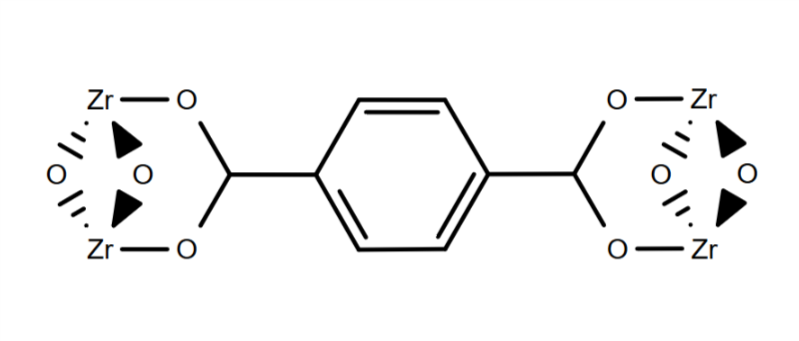
\includegraphics[width=0.3\linewidth]{structures/site-linker}}}\)%
    \( \longrightarrow \)%
    \(\vcenter{\hbox{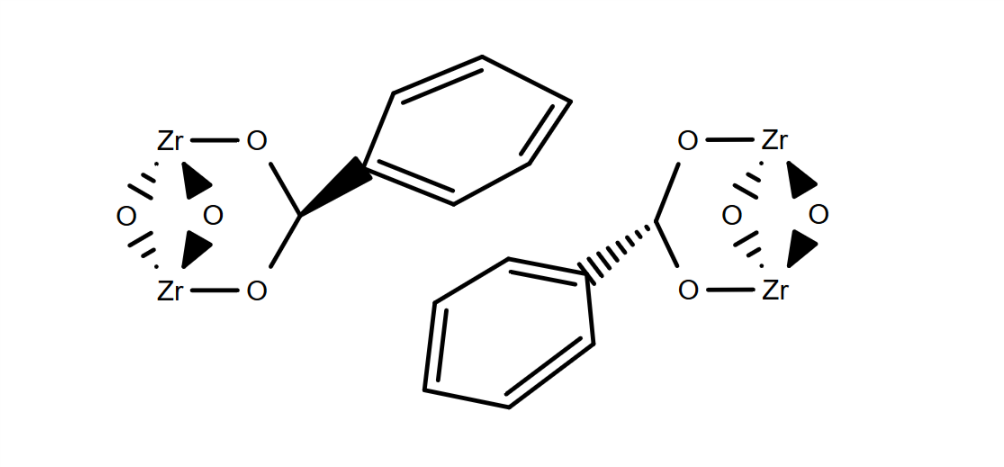
\includegraphics[width=0.4\linewidth]{structures/site-benzoic}}}\)
    \caption{A defect site created through benzoic acid.}%
    \label{def:fgr:benzoic-defect}
\end{figure}

The calculated pore sizes with both the HK method and the DFT method 
show two sharp peaks corresponding to the octahedral and tetrahedral
pores in the UiO-66 structure. In \autoref{def:fgr:psd}, the pore
size distribution for the DMSO dataset is depicted. The appearance of 
a tertiary pore is visible in the leached samples with formic,
acetic and trifluoroacetic acid. This pore size likely corresponds
to the increased pore volume introduced by missing linker-type 
defects. The calculated diameter of this tertiary pore is
inversely proportional to the molecular size of the 
leaching compound used, which is a clear indication of the presence of 
the acid molecules in the structure as capping agents. On the samples
which have been activated at \SI{320}{\degreeCelsius}, the pore width
shifts to a single value as the coordinated acids are evacuated.

The pore size distribution calculated in the benzoic acid leached
samples shows the disappearance of peaks larger than around 
\SI{1}{\nano\metre}, as the compound replaces formate as the 
capping agent for the initial defects in the structure. Due to the 
similarity of the terephtalate linker with benzoate, the structure
becomes more ``ideal'' than the pristine material. At high concentrations
of benzoic acid, an overall decrease in porosity may be seen, as 
two benzoate molecules may act as capping agents in adjacent 
sites as depicted in \autoref{def:fgr:benzoic-defect}, effectively 
lowering the available pore volume. The effect is corroborated 
by trends in the linker-to-node ratio, surface area and total 
pore volume in both methanol, DMSO and to a lesser extent DMF. 

At very high concentrations of TFA and BA, a fourth pore size
begins to be appear in the DFT calculated pore distribution.
This is likely evidence that missing cluster defects can be 
introduced at these concentrations. It should be noted that 
if such large-scale modifications of the structure are possible,
complete structural breakdown is not far away. Indeed, samples with 
higher concentrations of acid could not be obtained with TFA in DMSO,
with sample subjected to these conditions ending up completely
dissolved.


\begin{figure}[!h]
    \centering

    \begin{subfigure}{0.25\linewidth}
        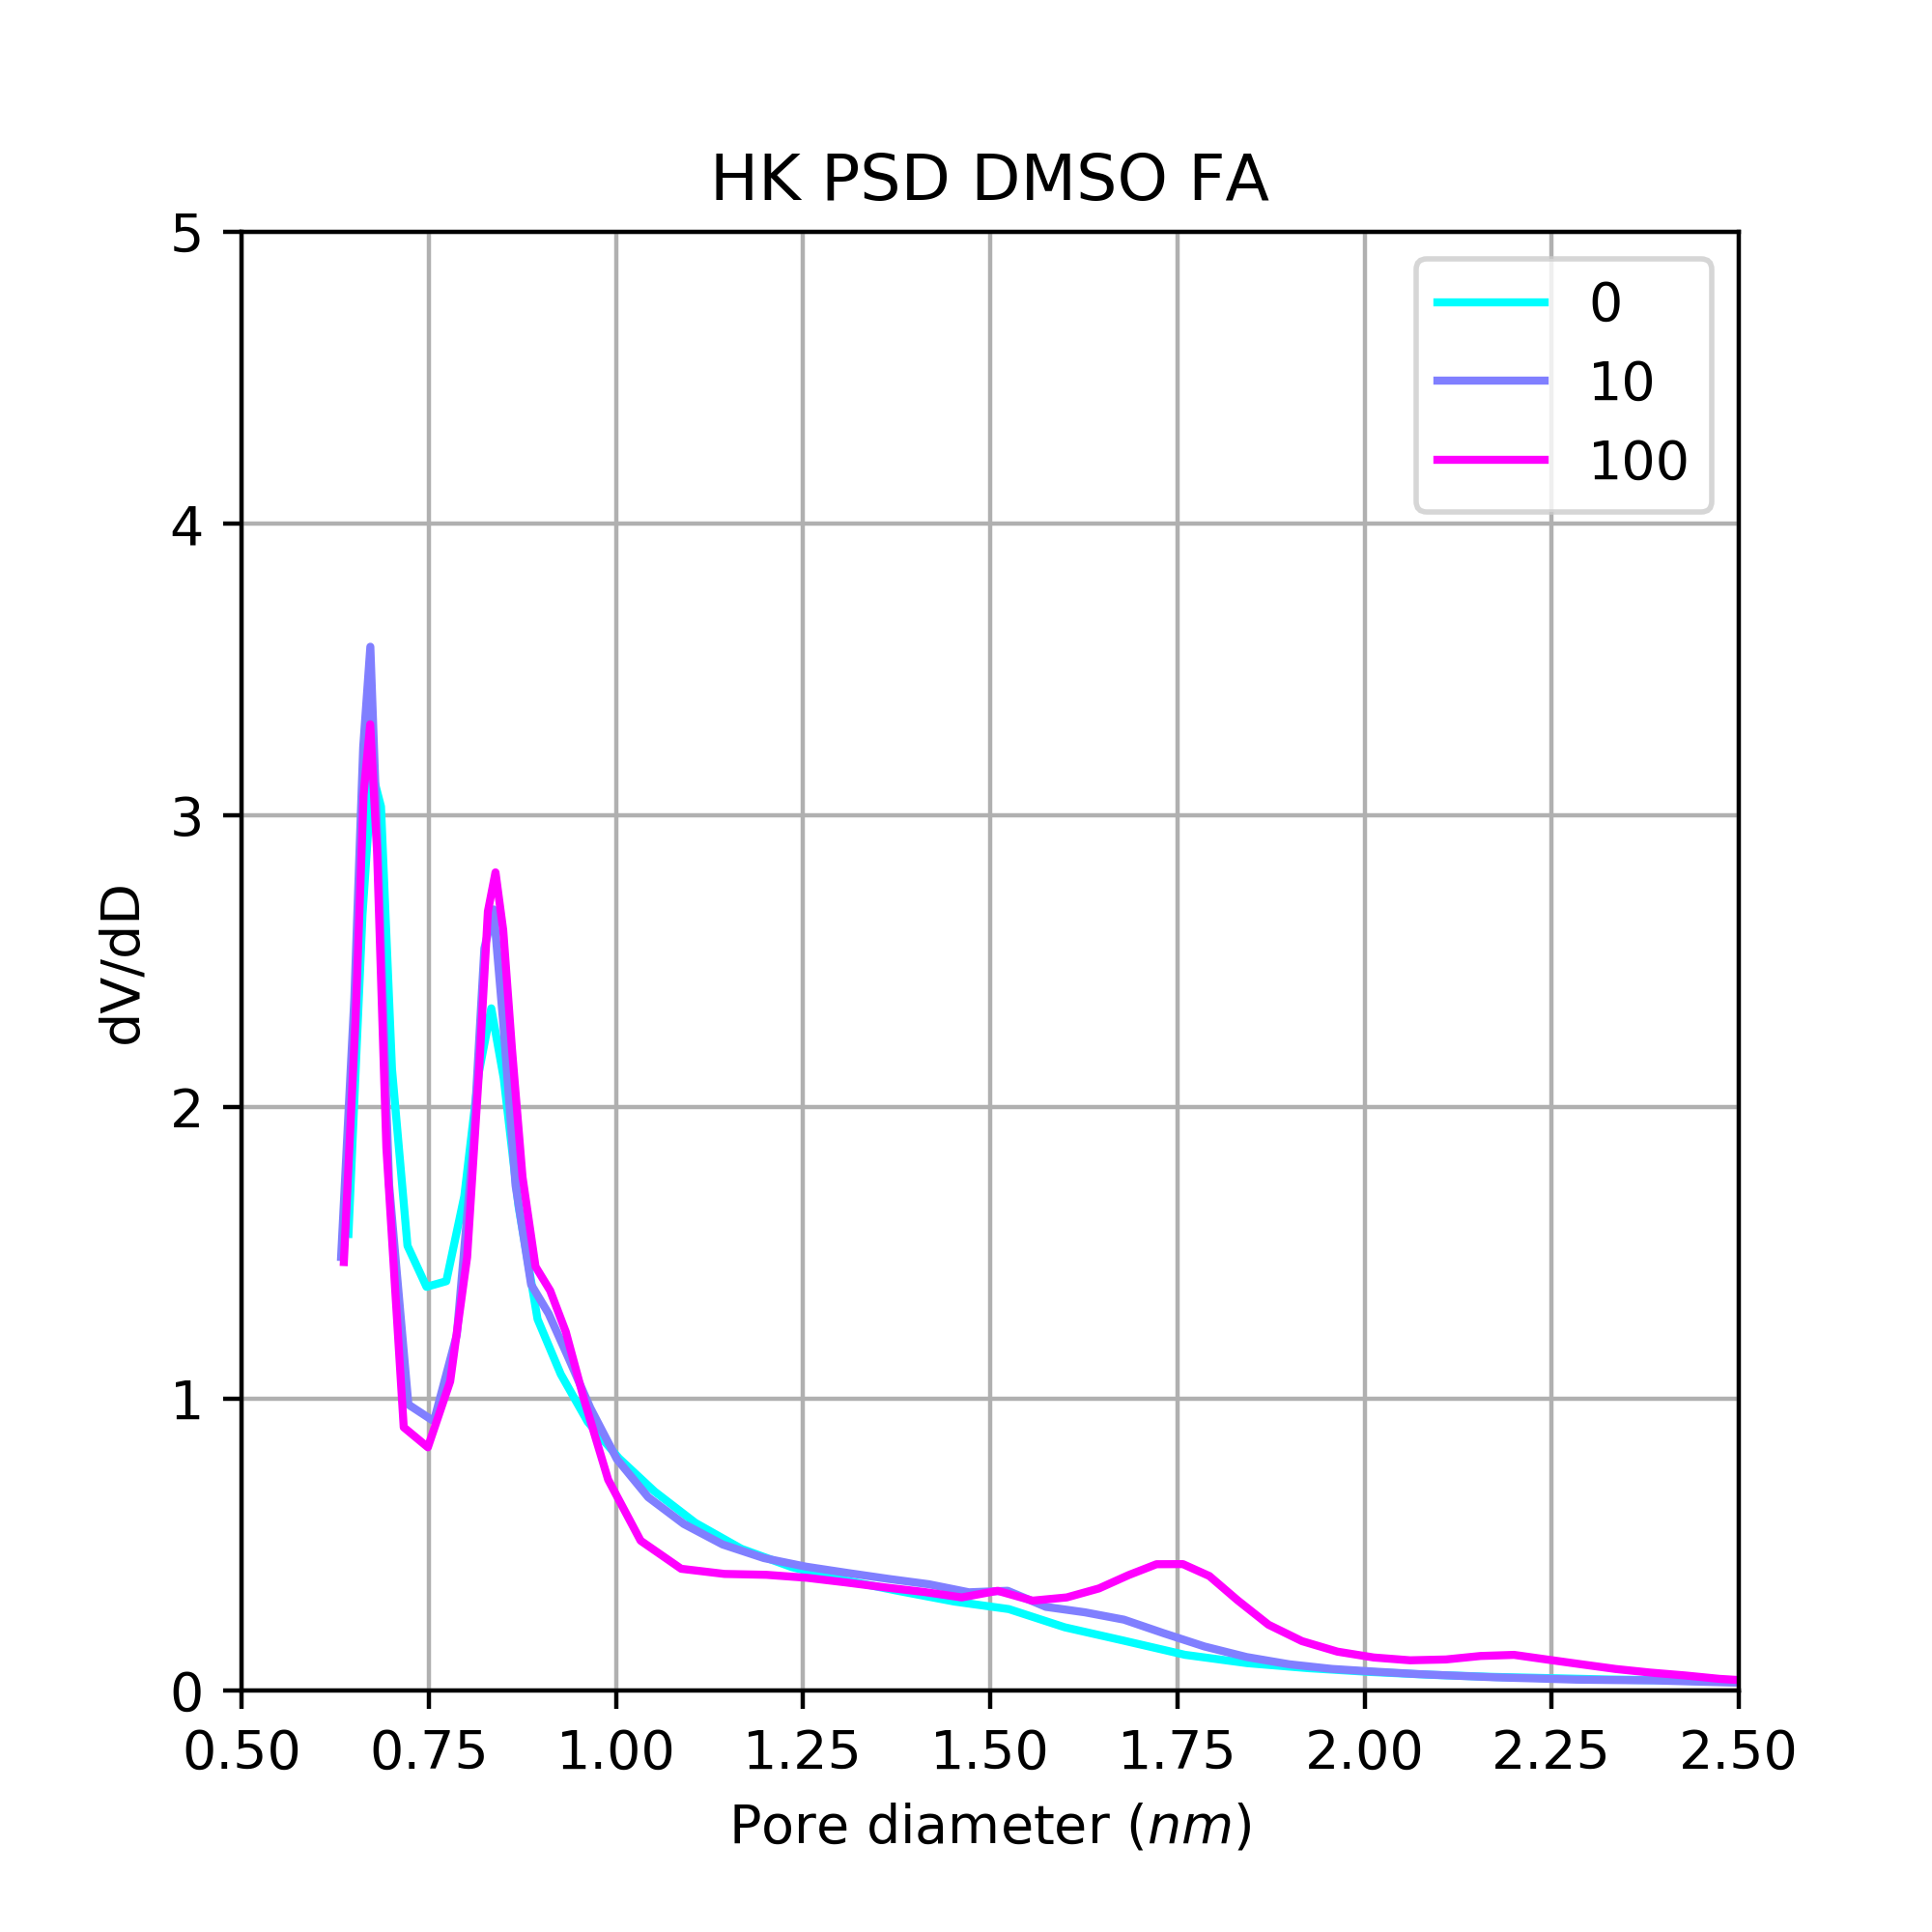
\includegraphics[width=\textwidth]{n2phys/dmso-fa-psd-hk}%
        \label{def:fgr:psd-dmso-fa-hk}
    \end{subfigure}%
    \begin{subfigure}{0.25\linewidth}
        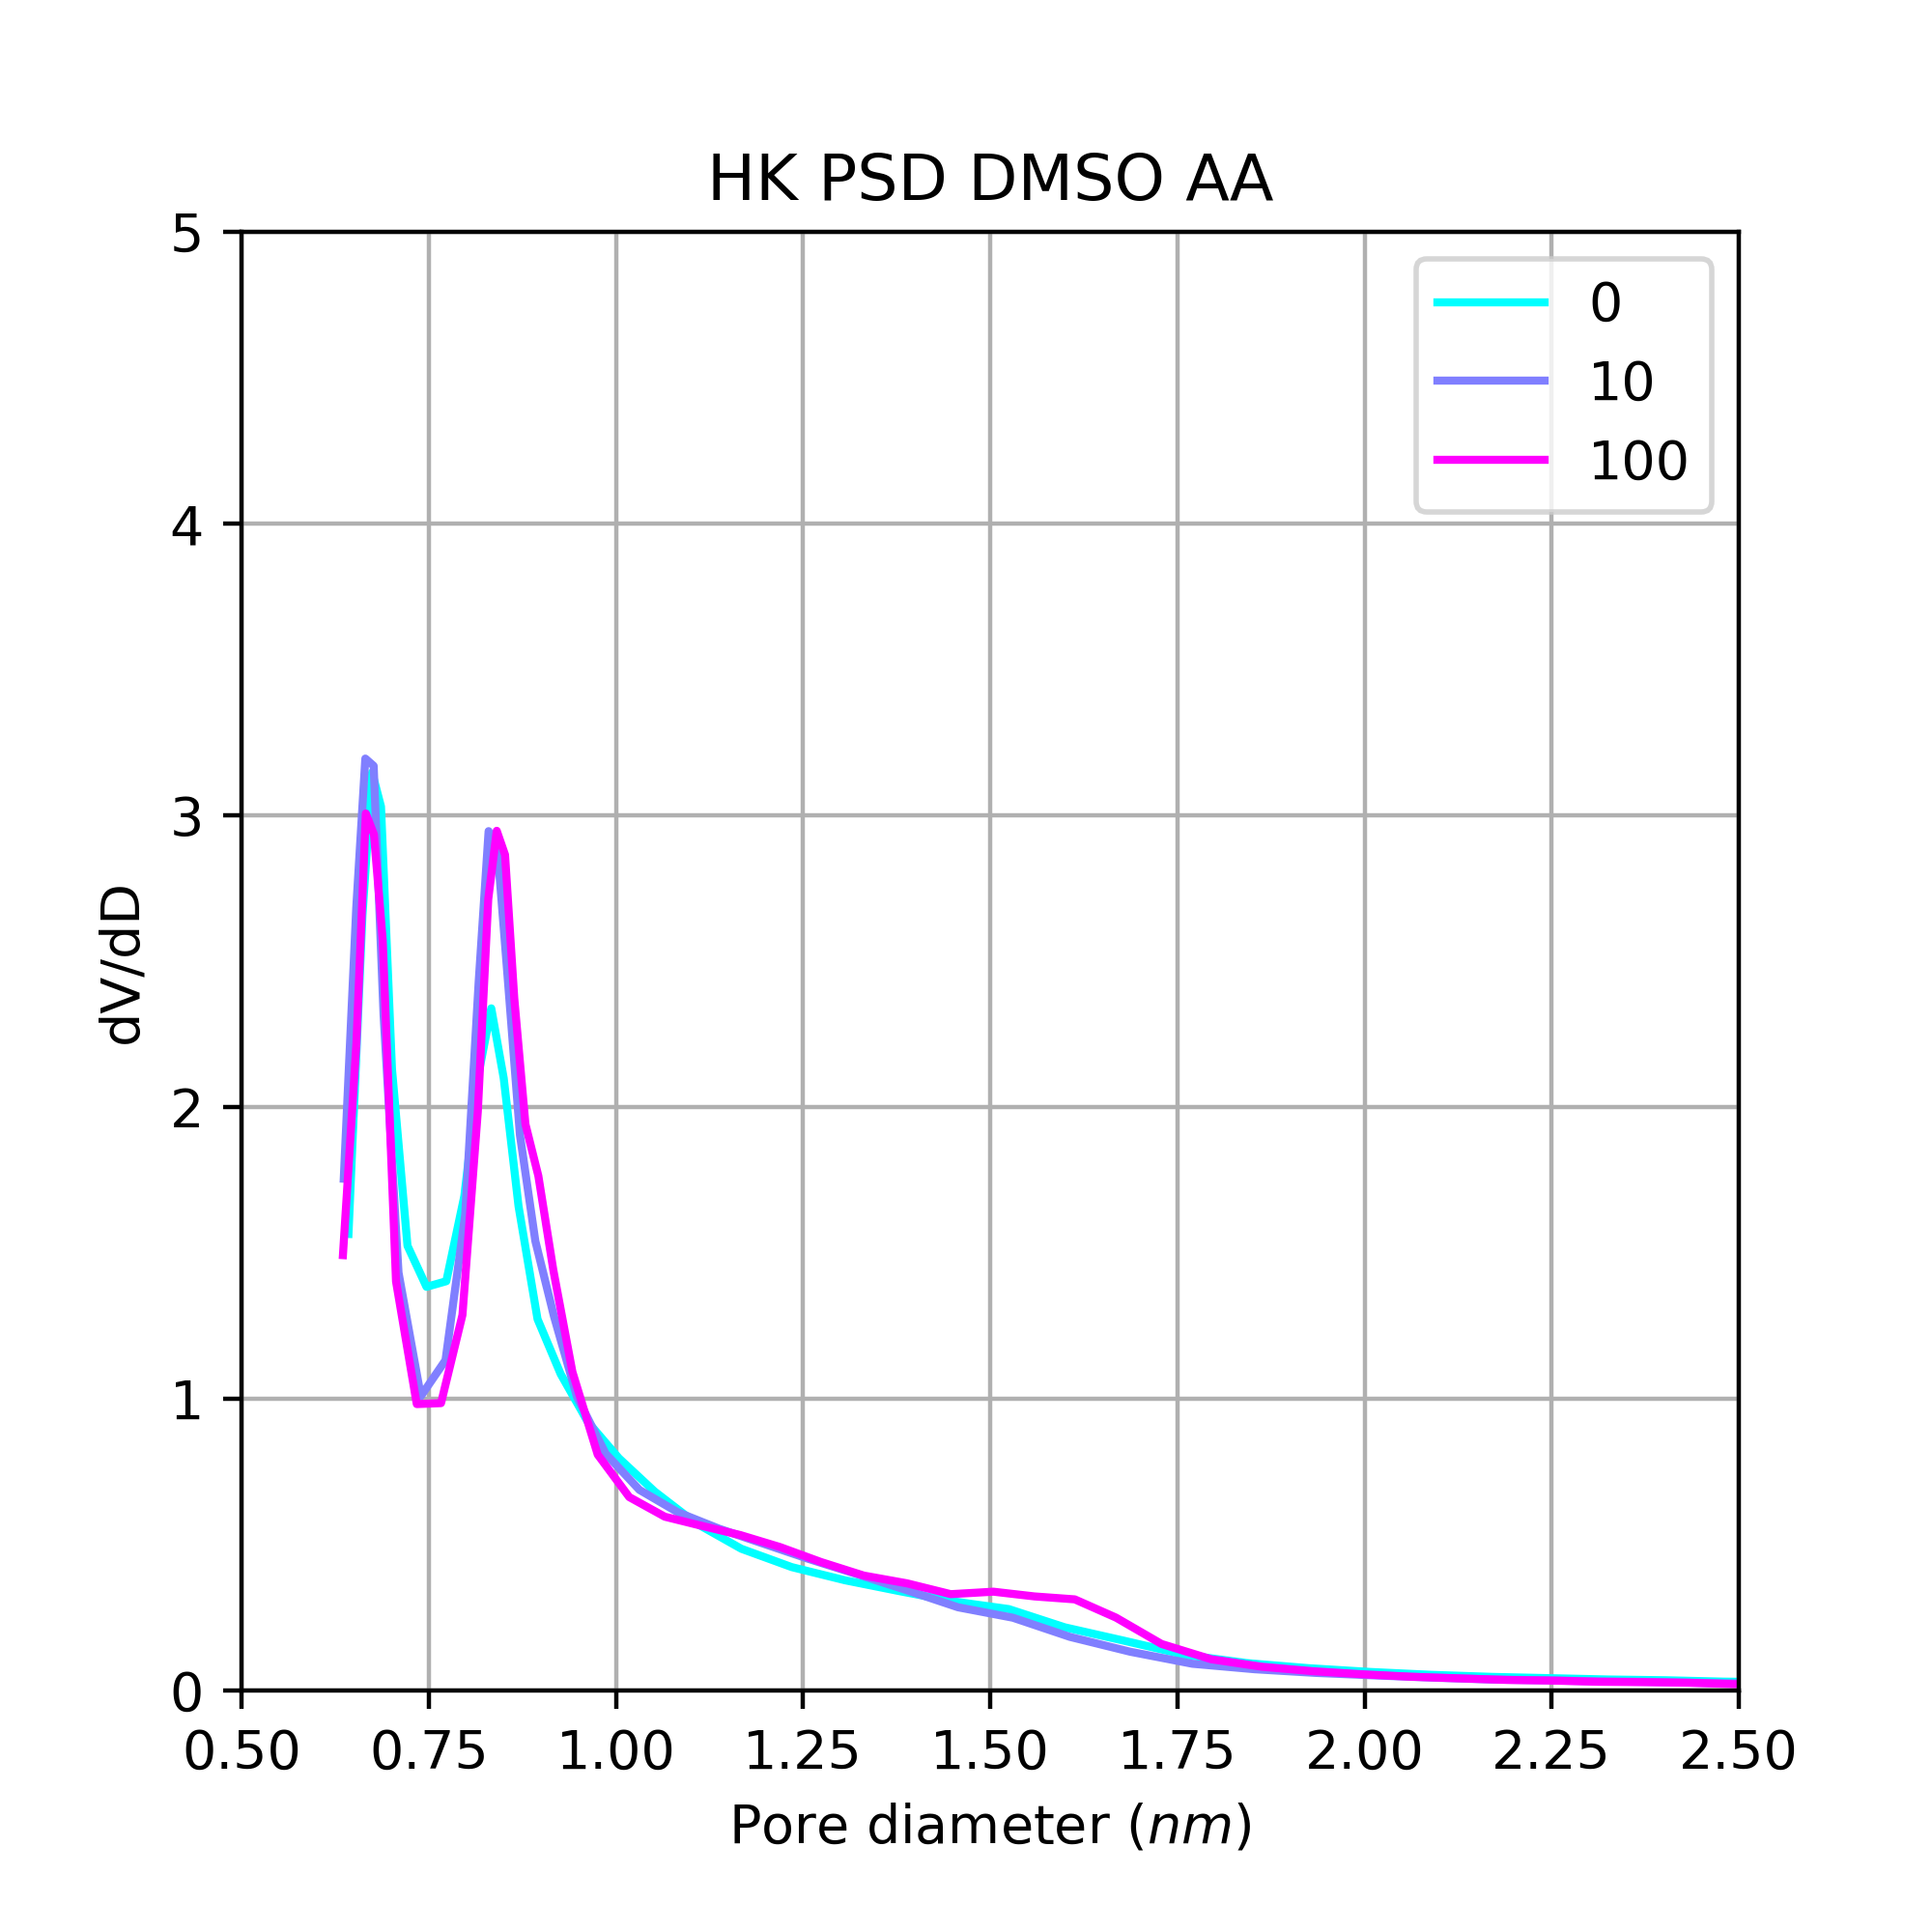
\includegraphics[width=\textwidth]{n2phys/dmso-aa-psd-hk}%
        \label{def:fgr:psd-dmso-aa-hk}
    \end{subfigure}%
    \begin{subfigure}{0.25\linewidth}
        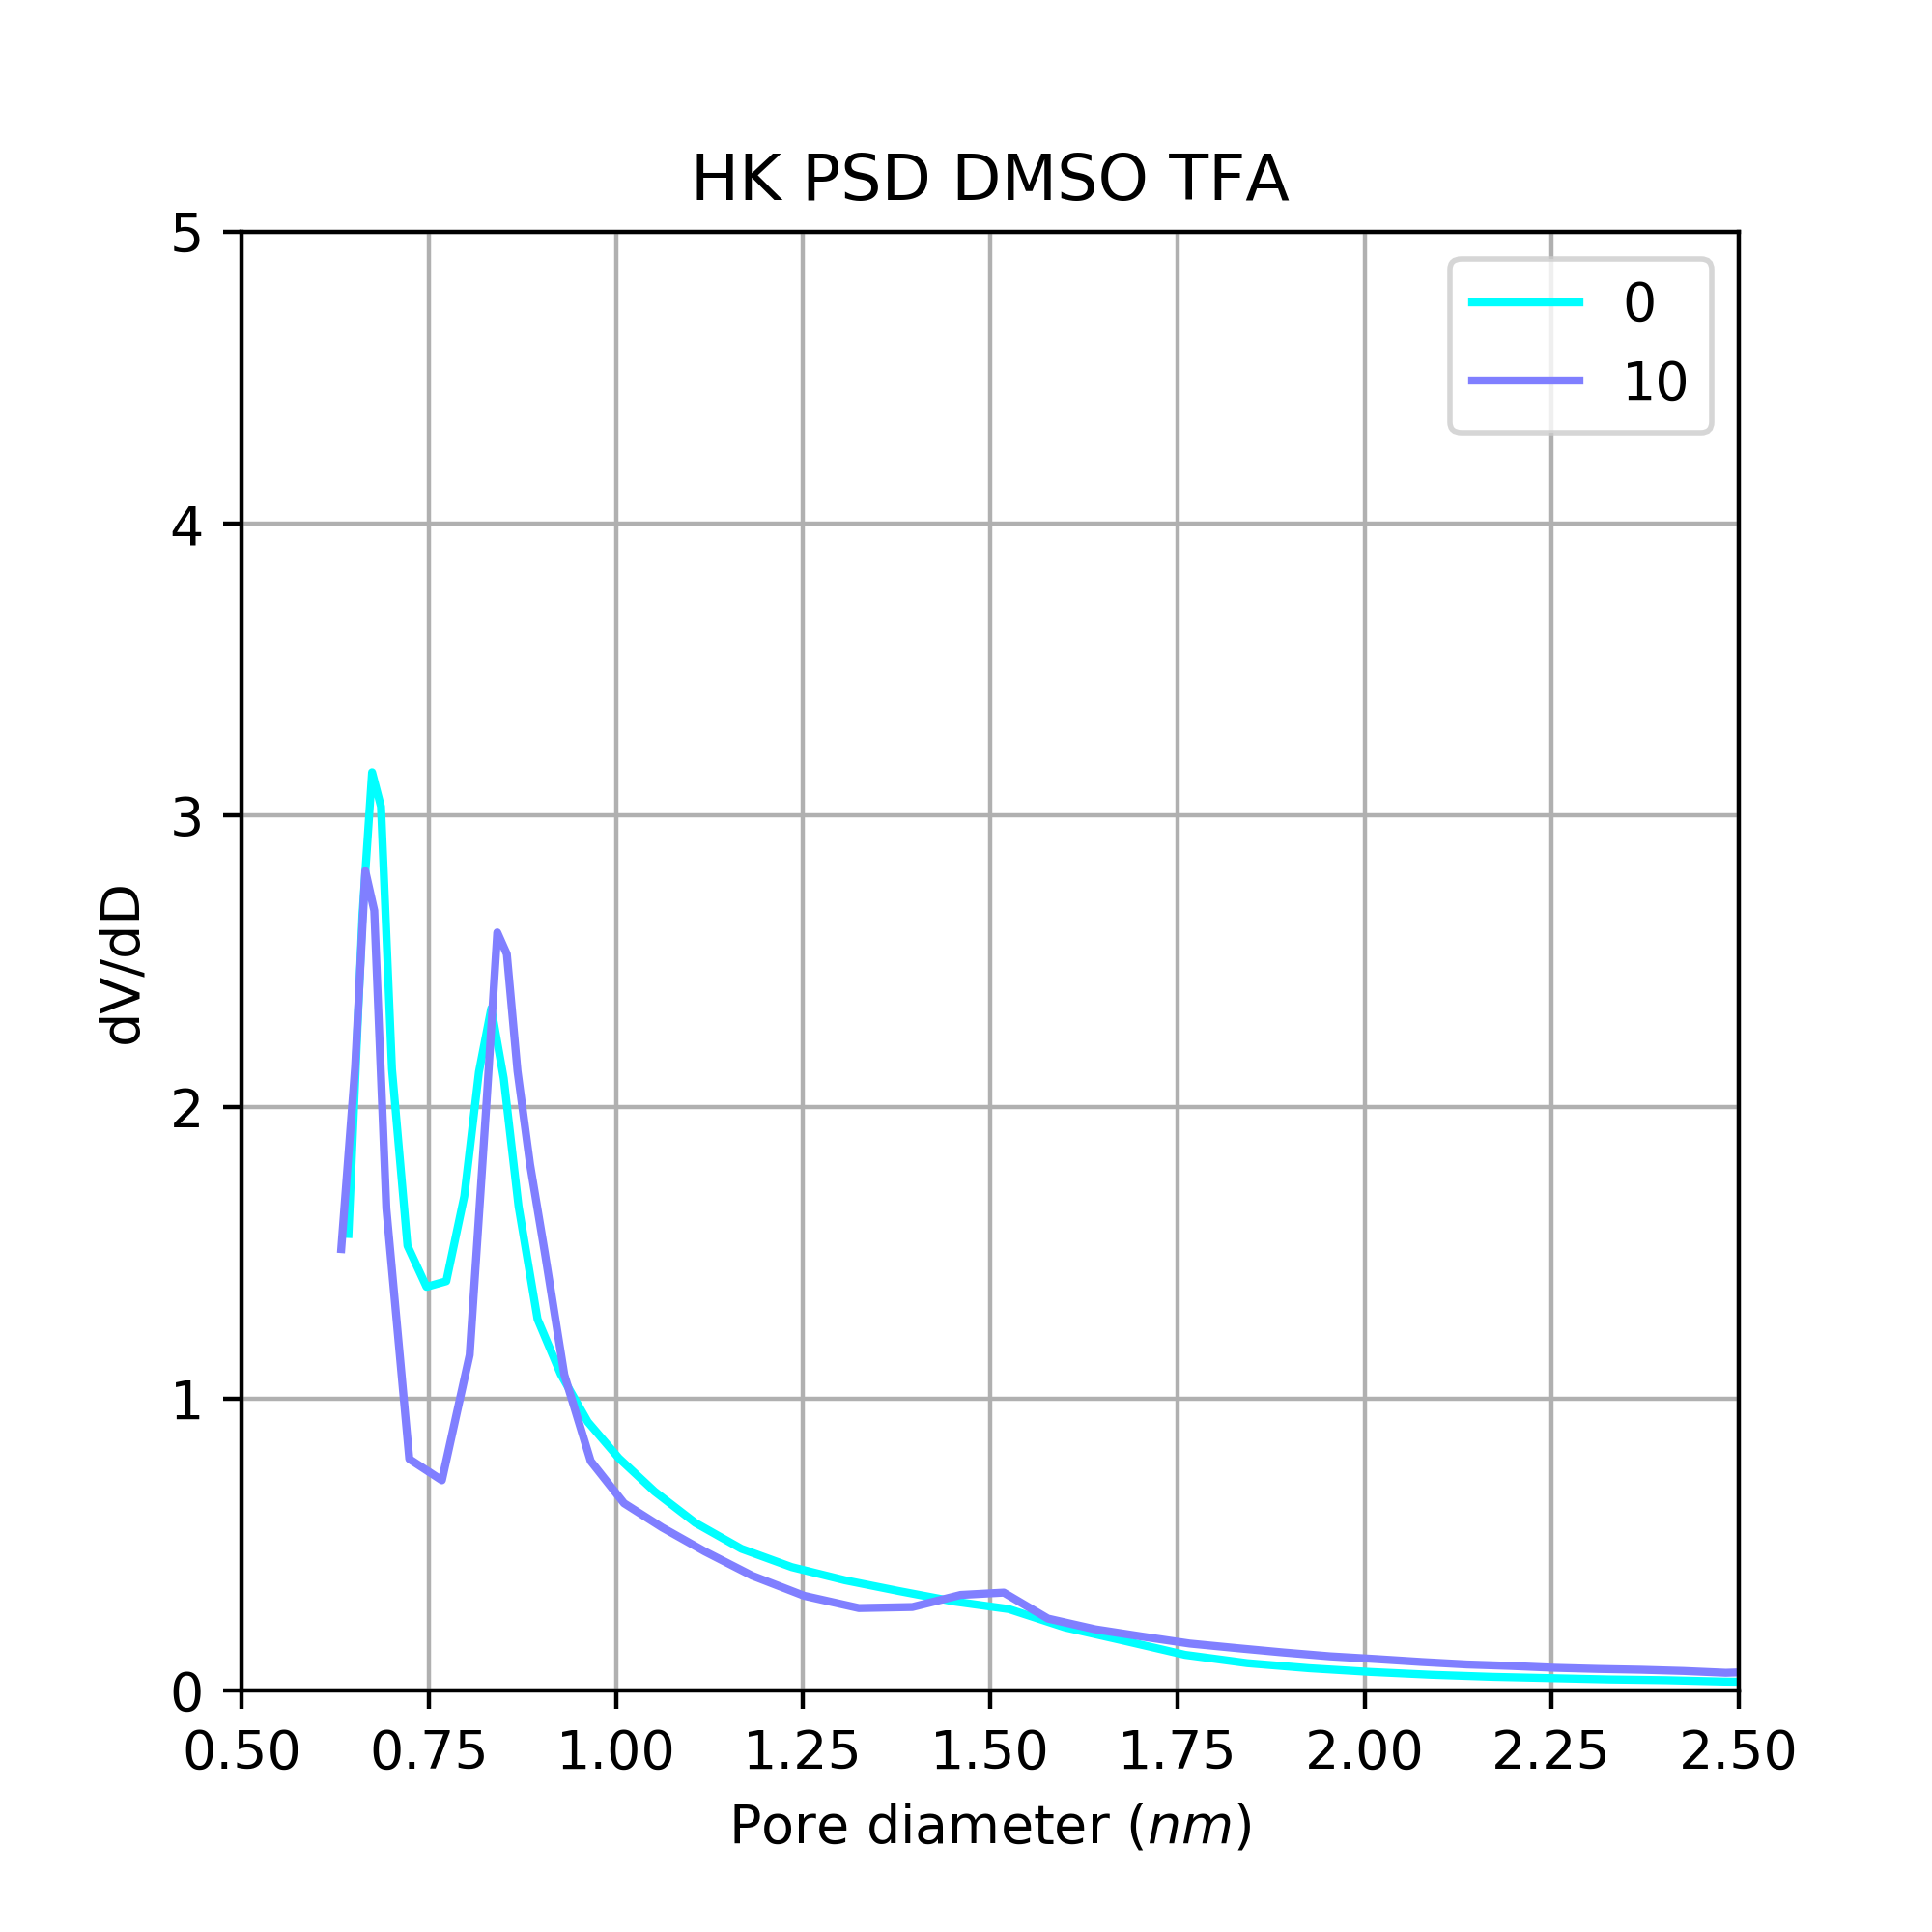
\includegraphics[width=\textwidth]{n2phys/dmso-tfa-psd-hk}%
        \label{def:fgr:psd-dmso-tfa-hk}
    \end{subfigure}%
    \begin{subfigure}{0.25\linewidth}
        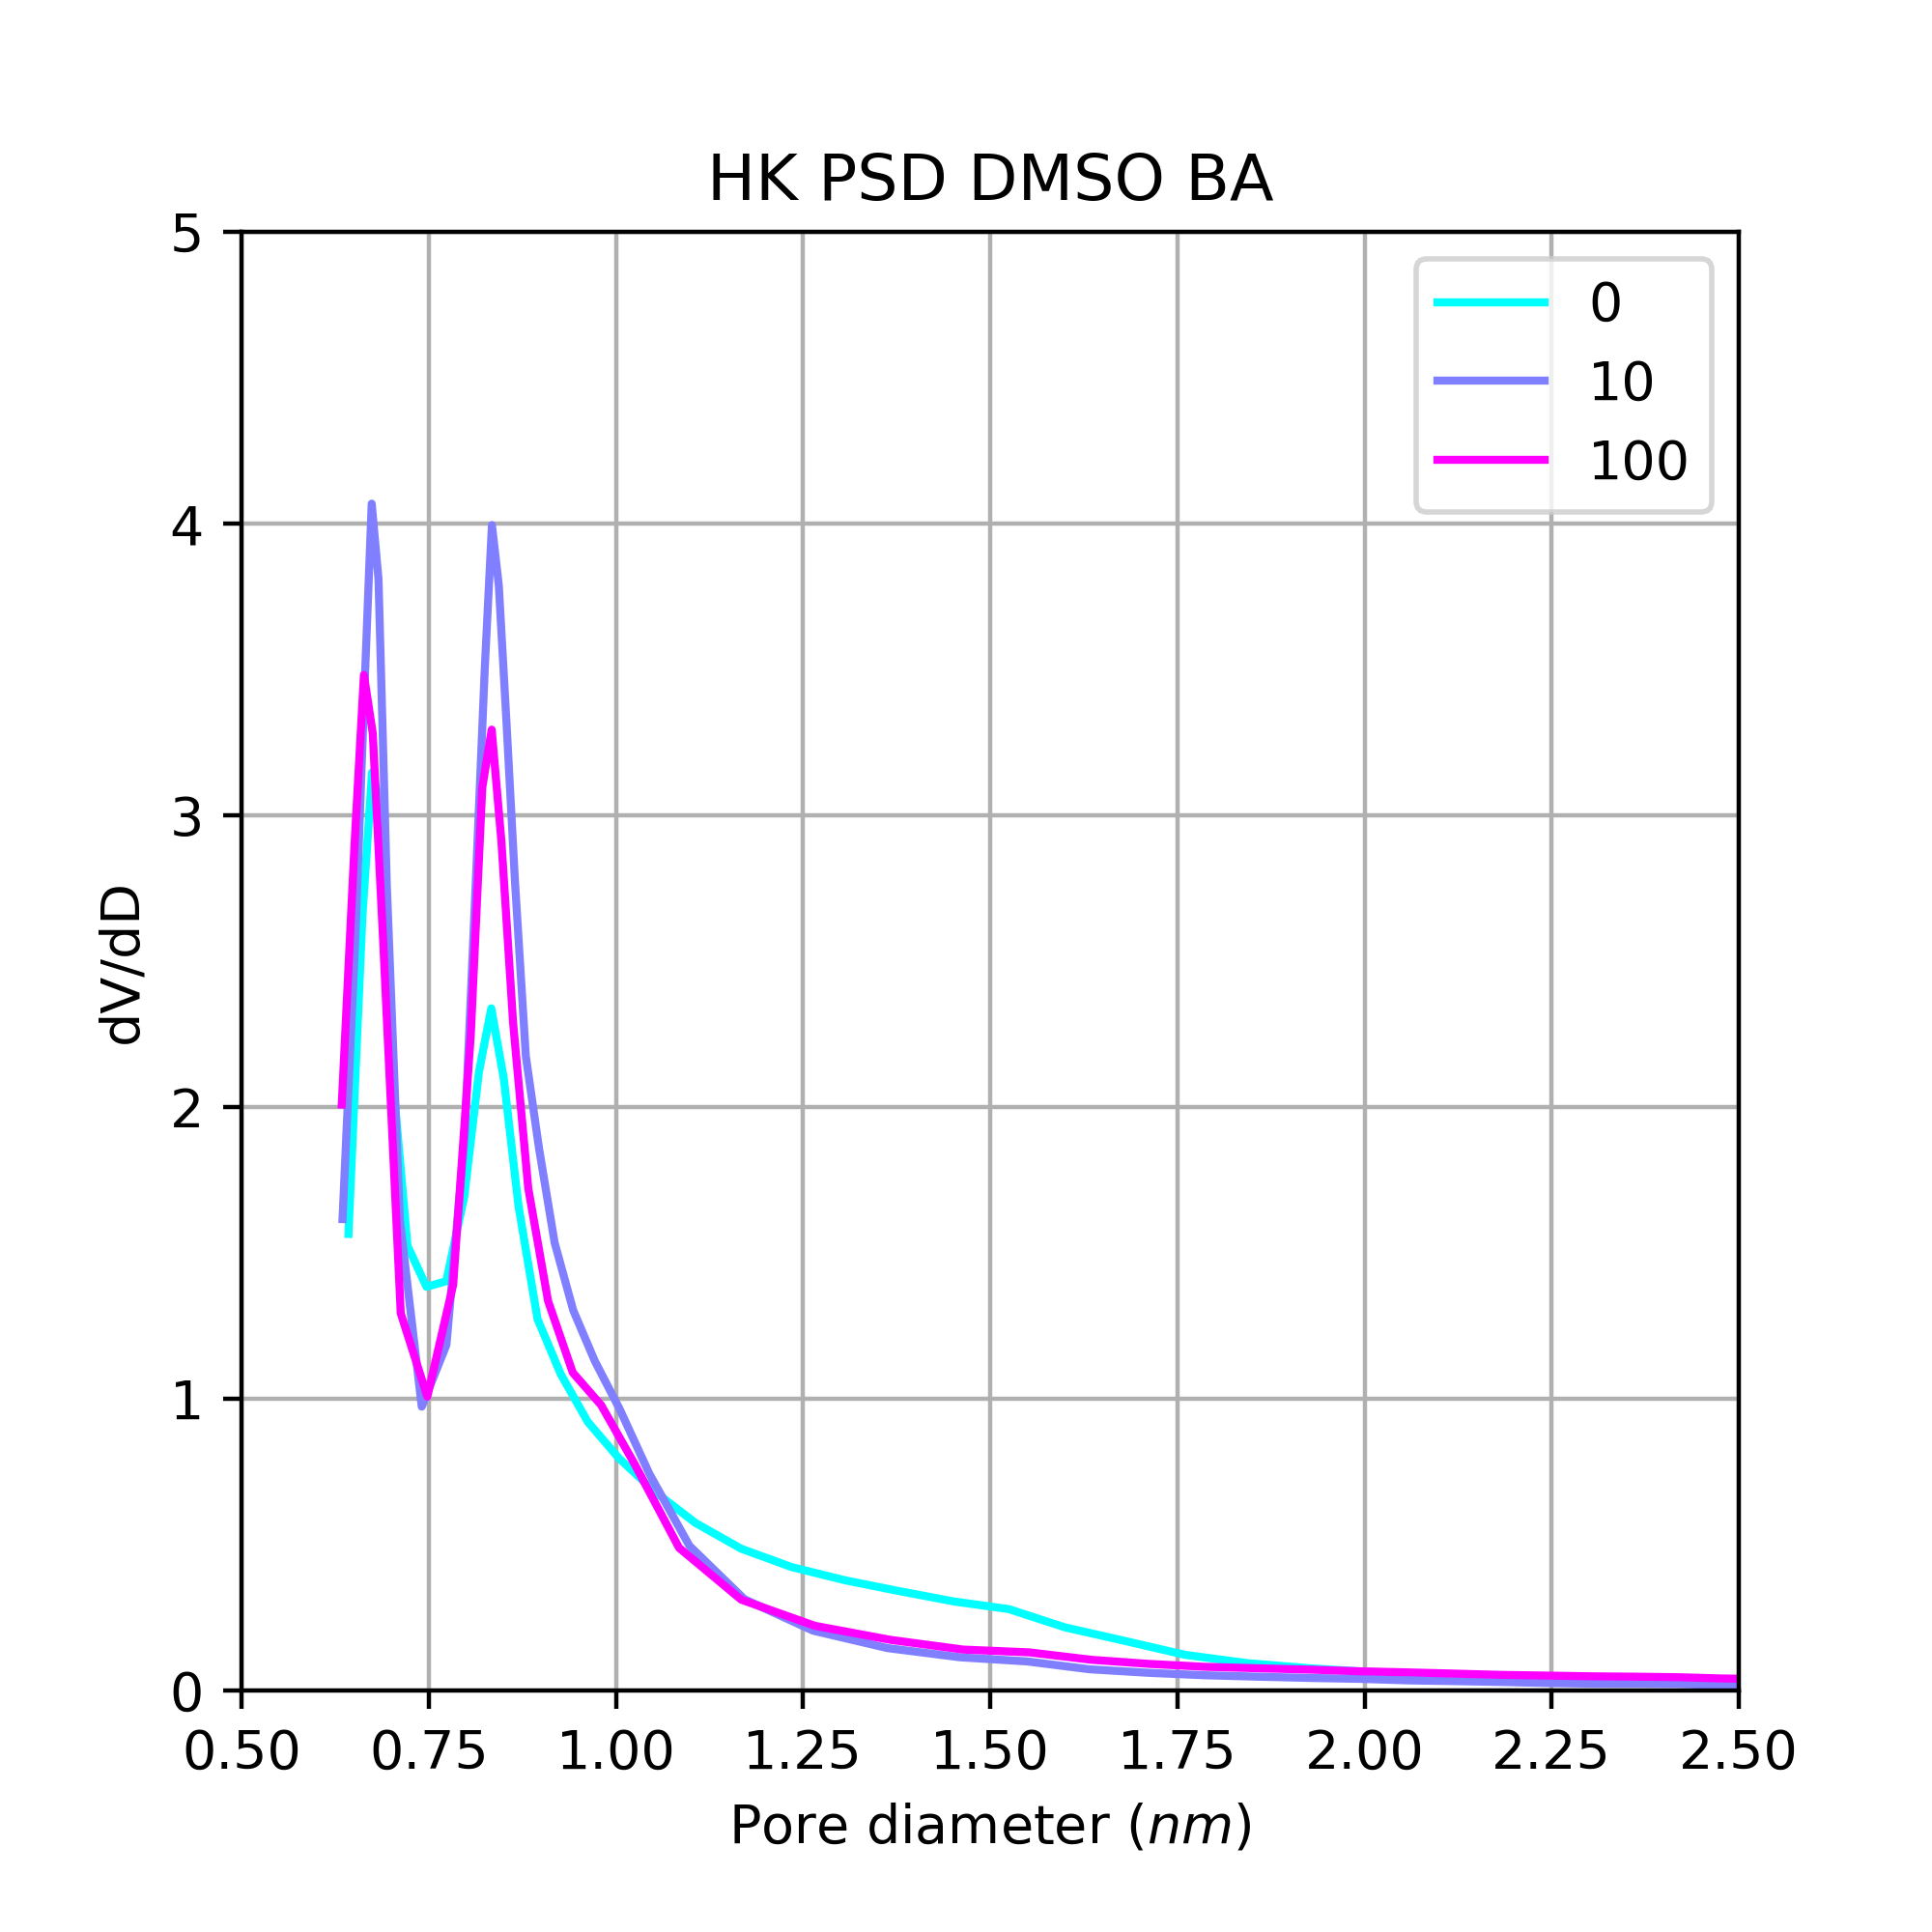
\includegraphics[width=\textwidth]{n2phys/dmso-ba-psd-hk}%
        \label{def:fgr:psd-dmso-ba-hk}
    \end{subfigure}%

    \begin{subfigure}{0.25\linewidth}
        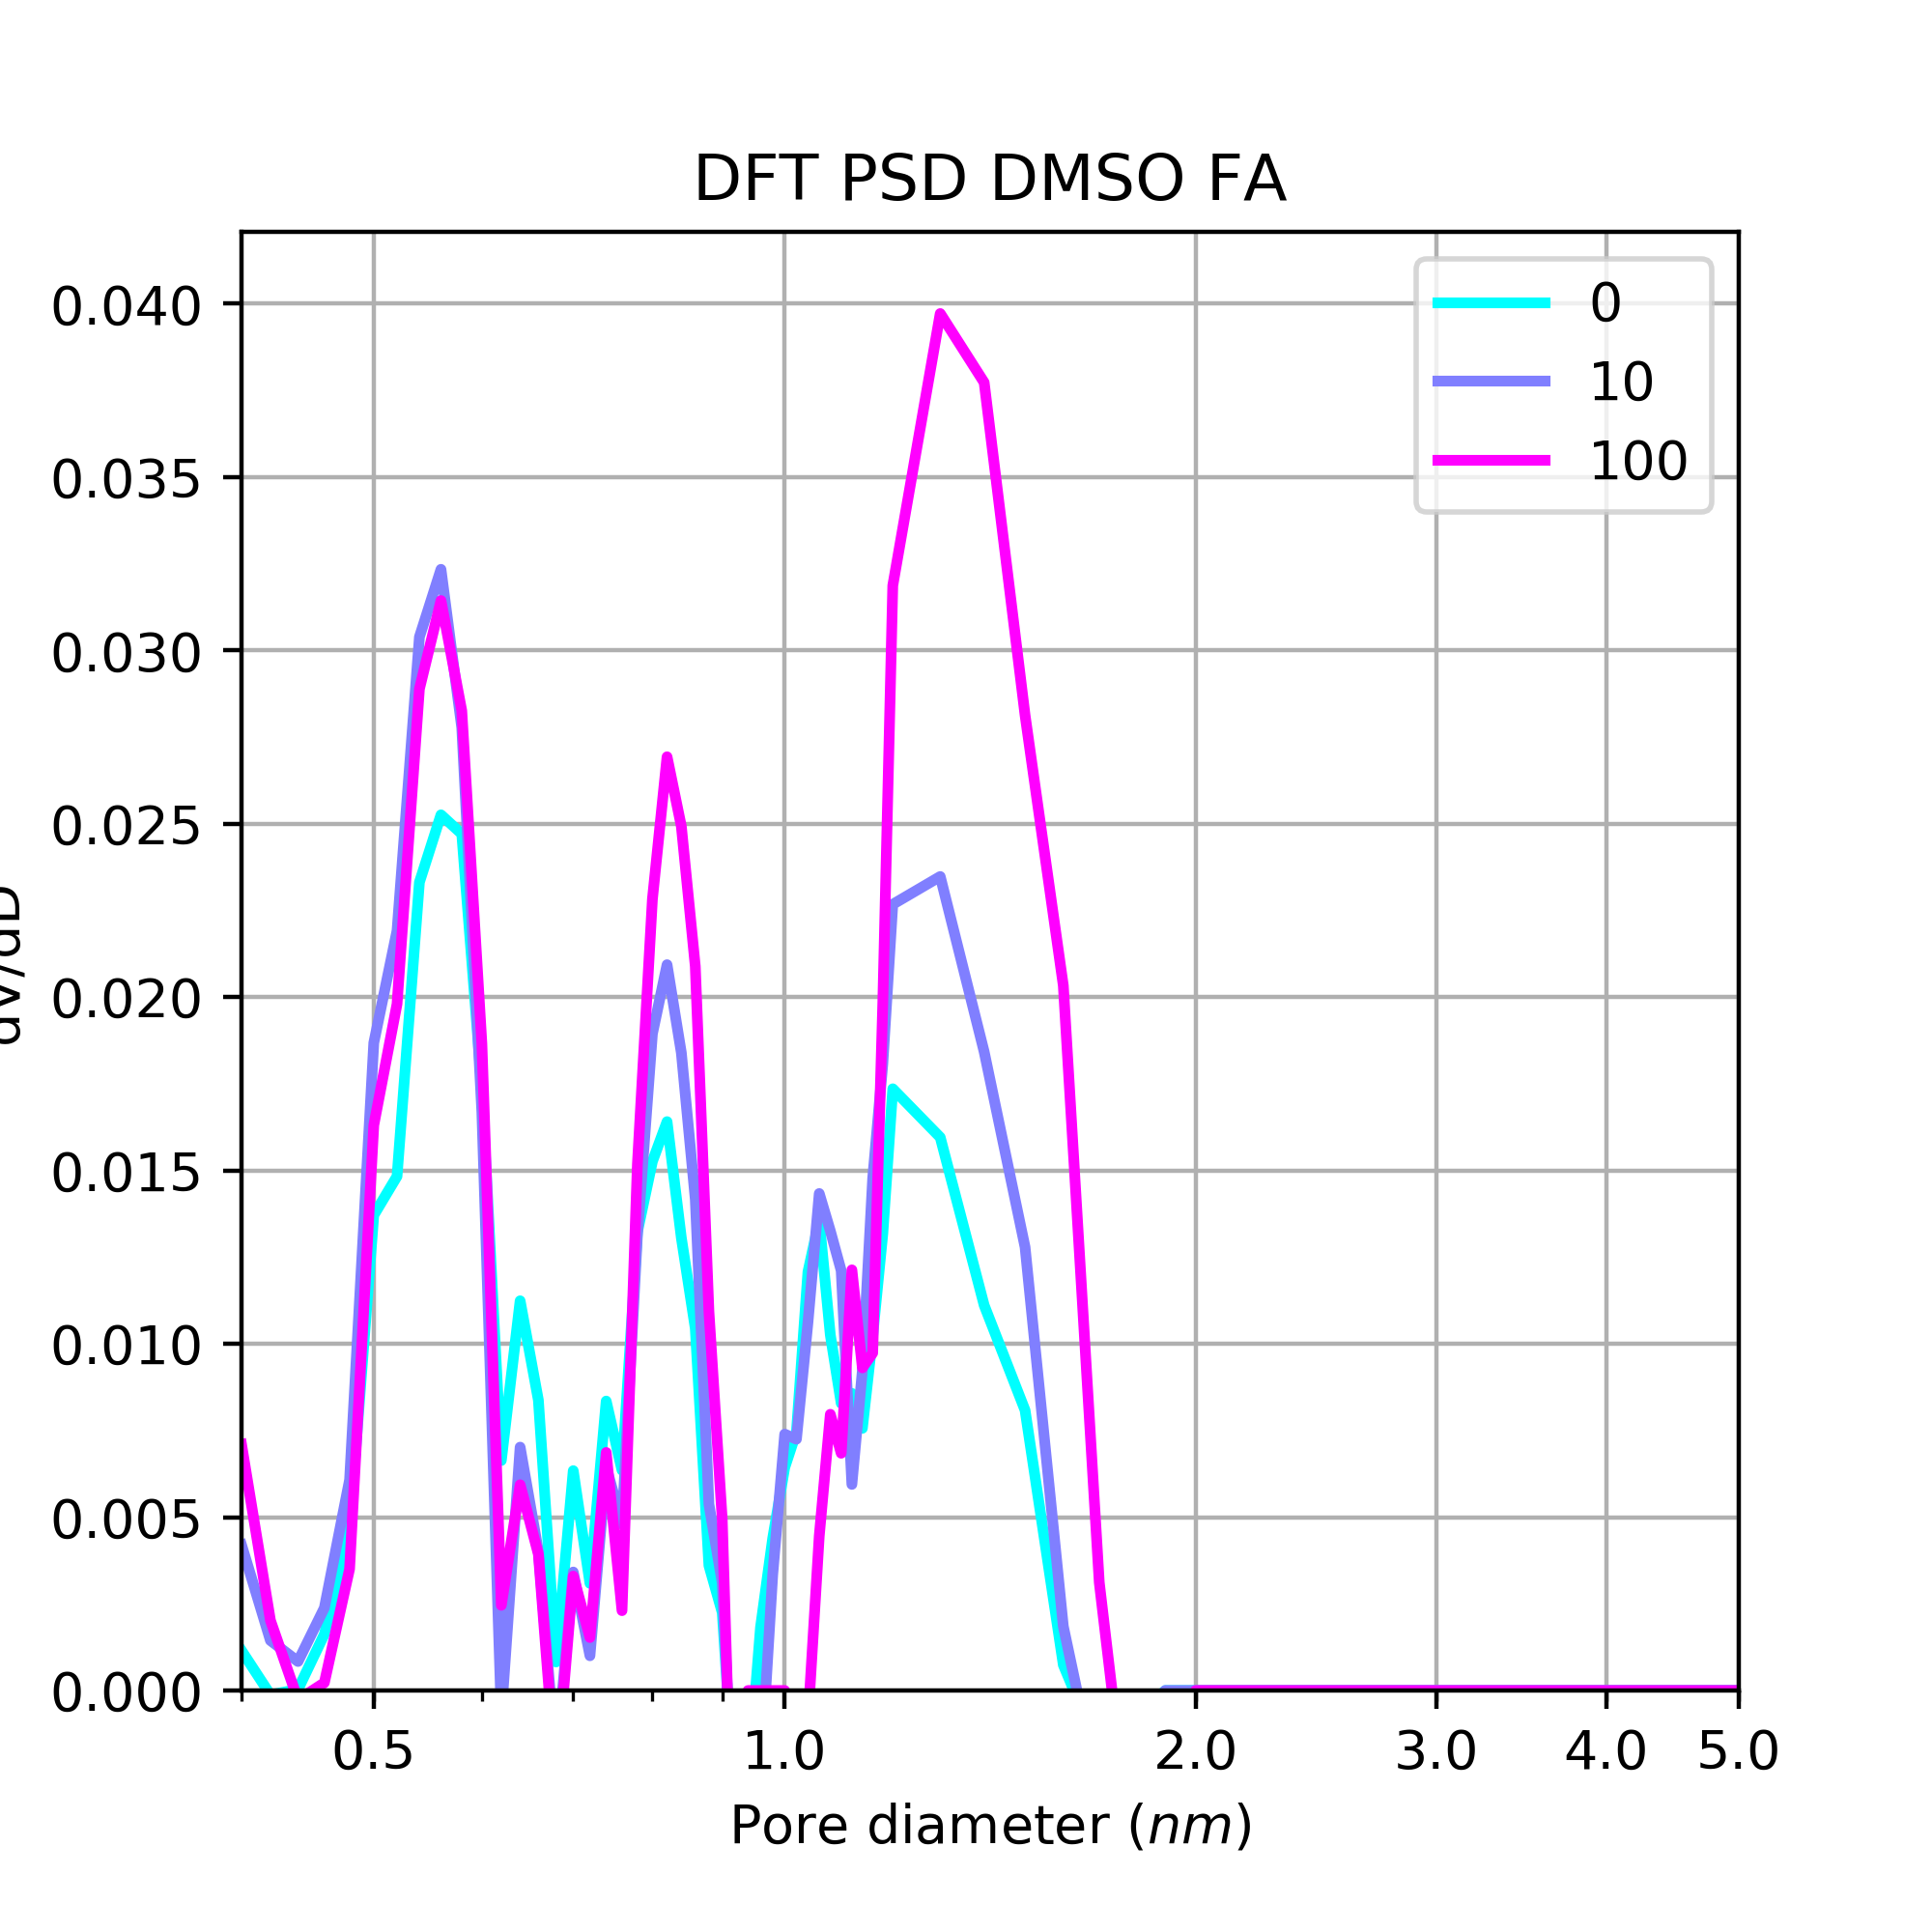
\includegraphics[width=\textwidth]{n2phys/dmso-fa-psd-dft}%
        \label{def:fgr:psd-dmso-fa-dft}
    \end{subfigure}%
    \begin{subfigure}{0.25\linewidth}
        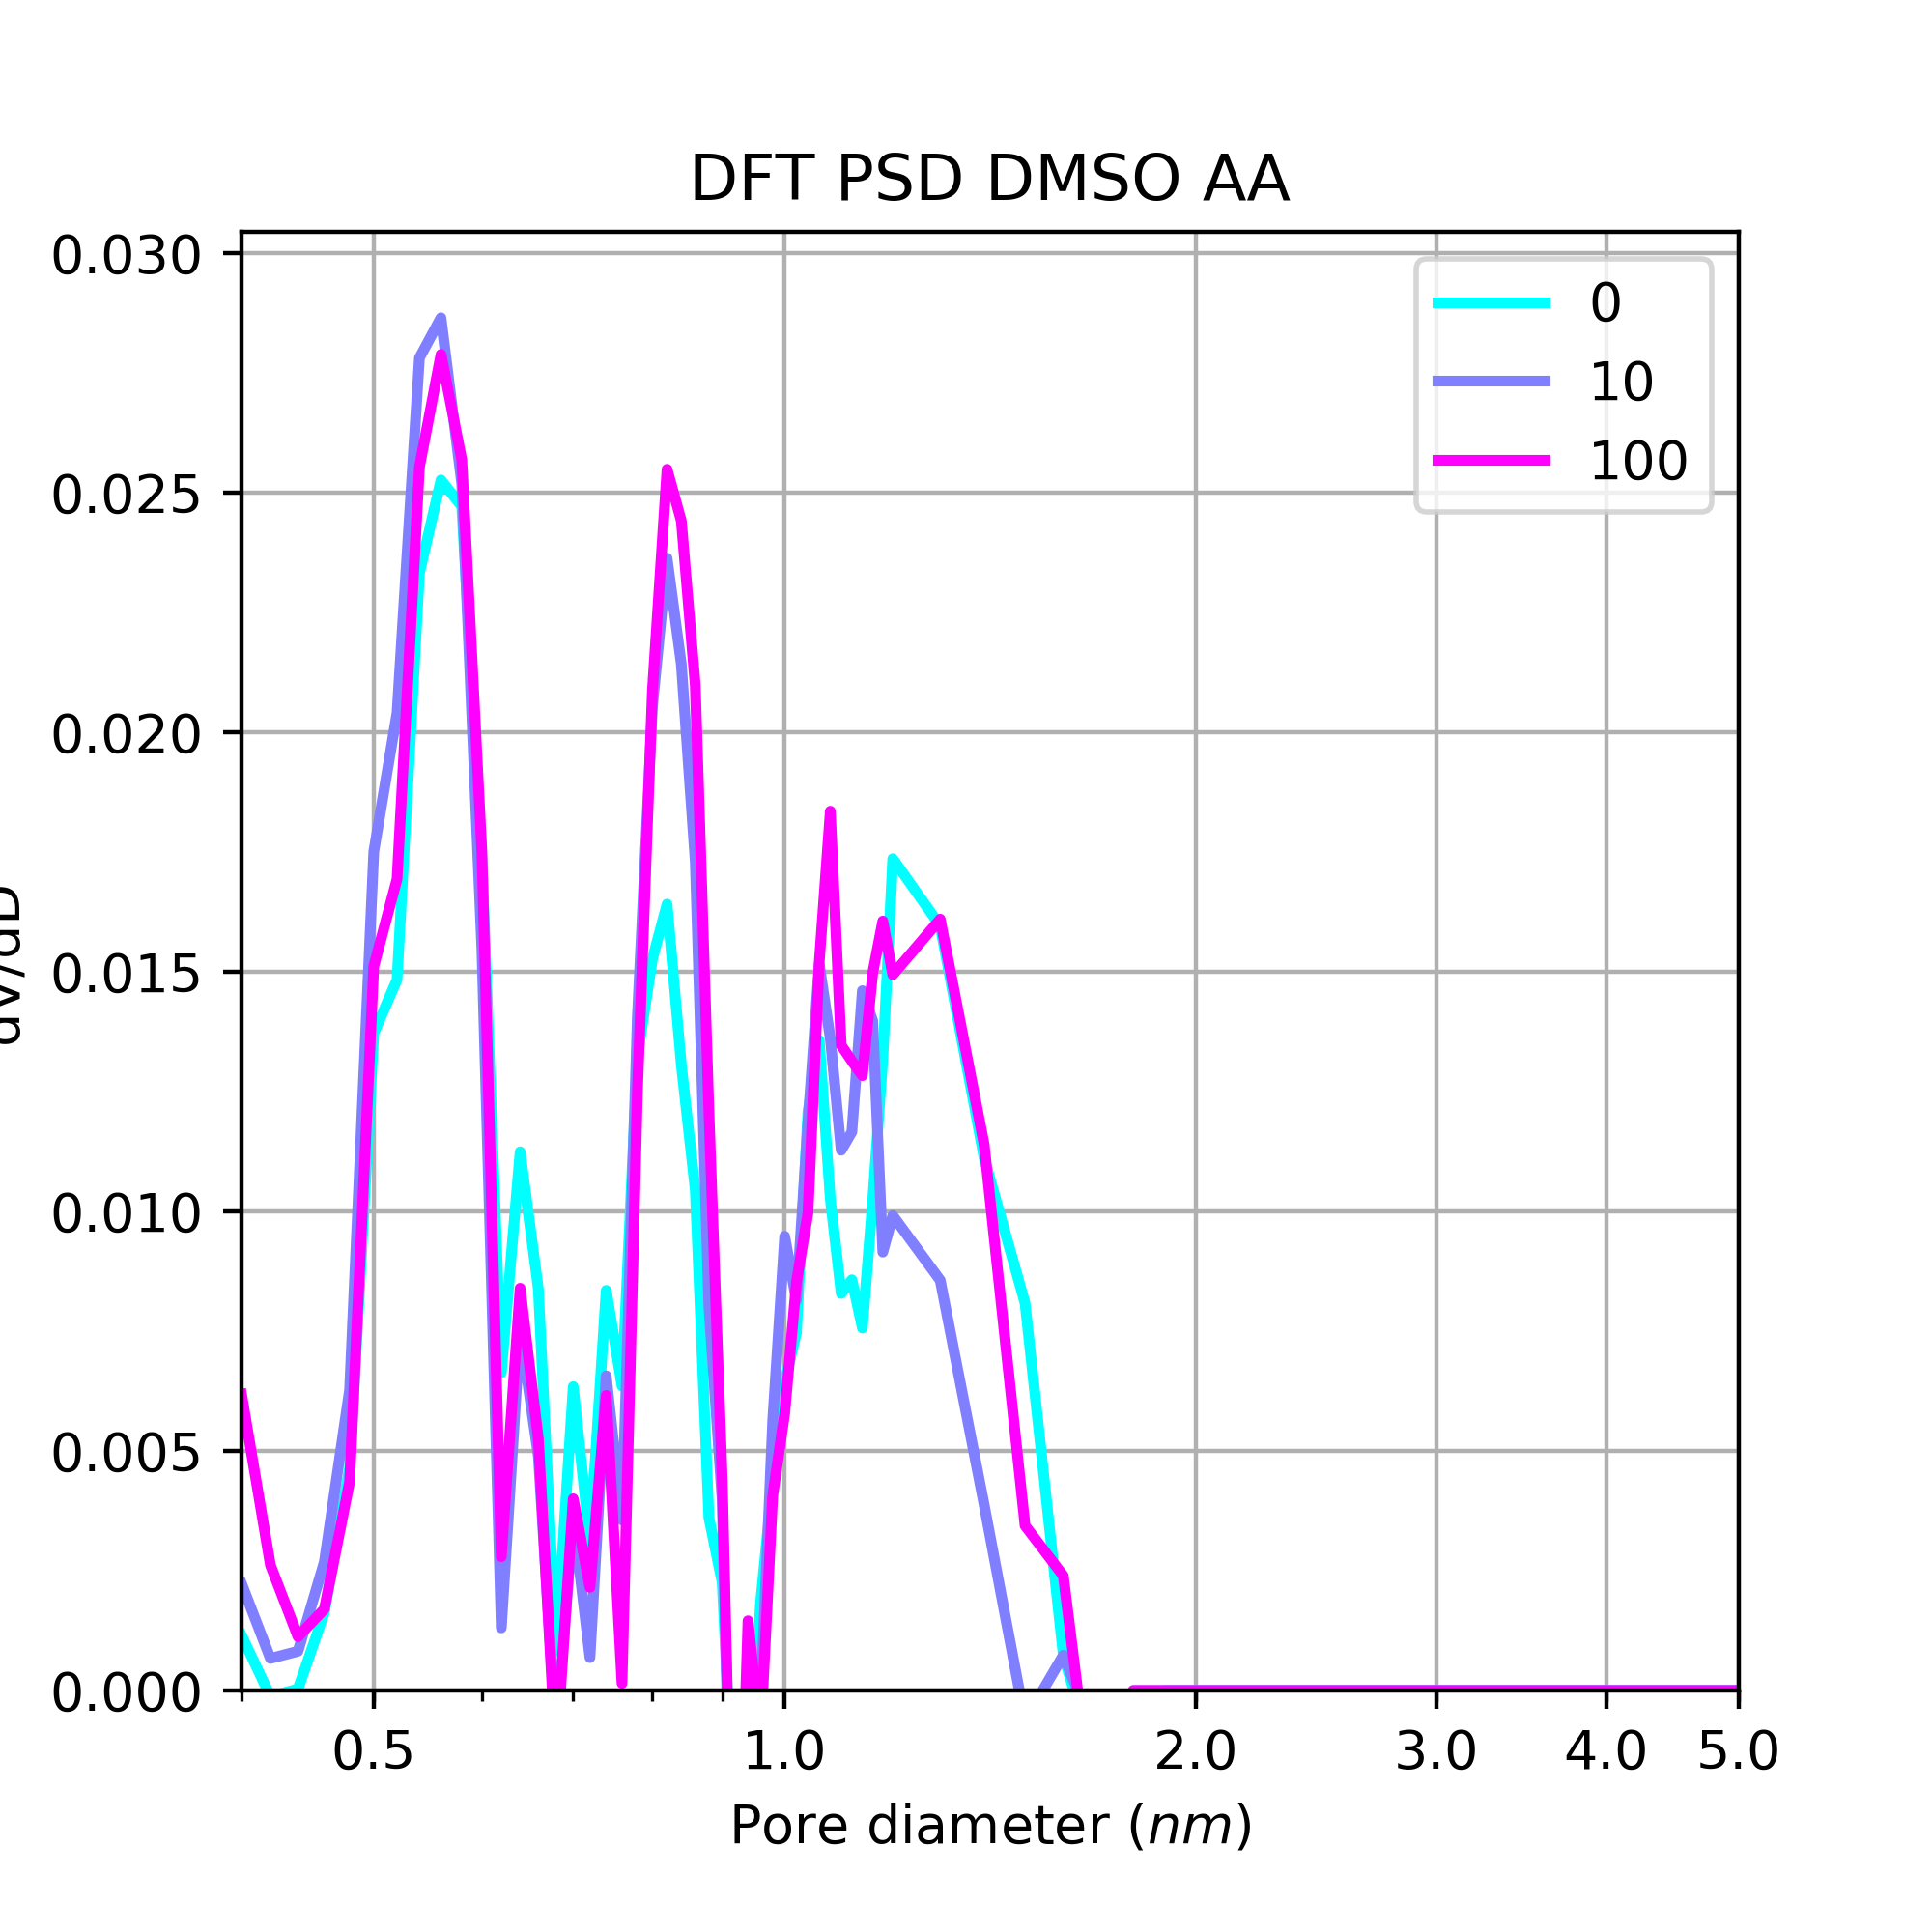
\includegraphics[width=\textwidth]{n2phys/dmso-aa-psd-dft}%
        \label{def:fgr:psd-dmso-aa-dft}
    \end{subfigure}%
    \begin{subfigure}{0.25\linewidth}
        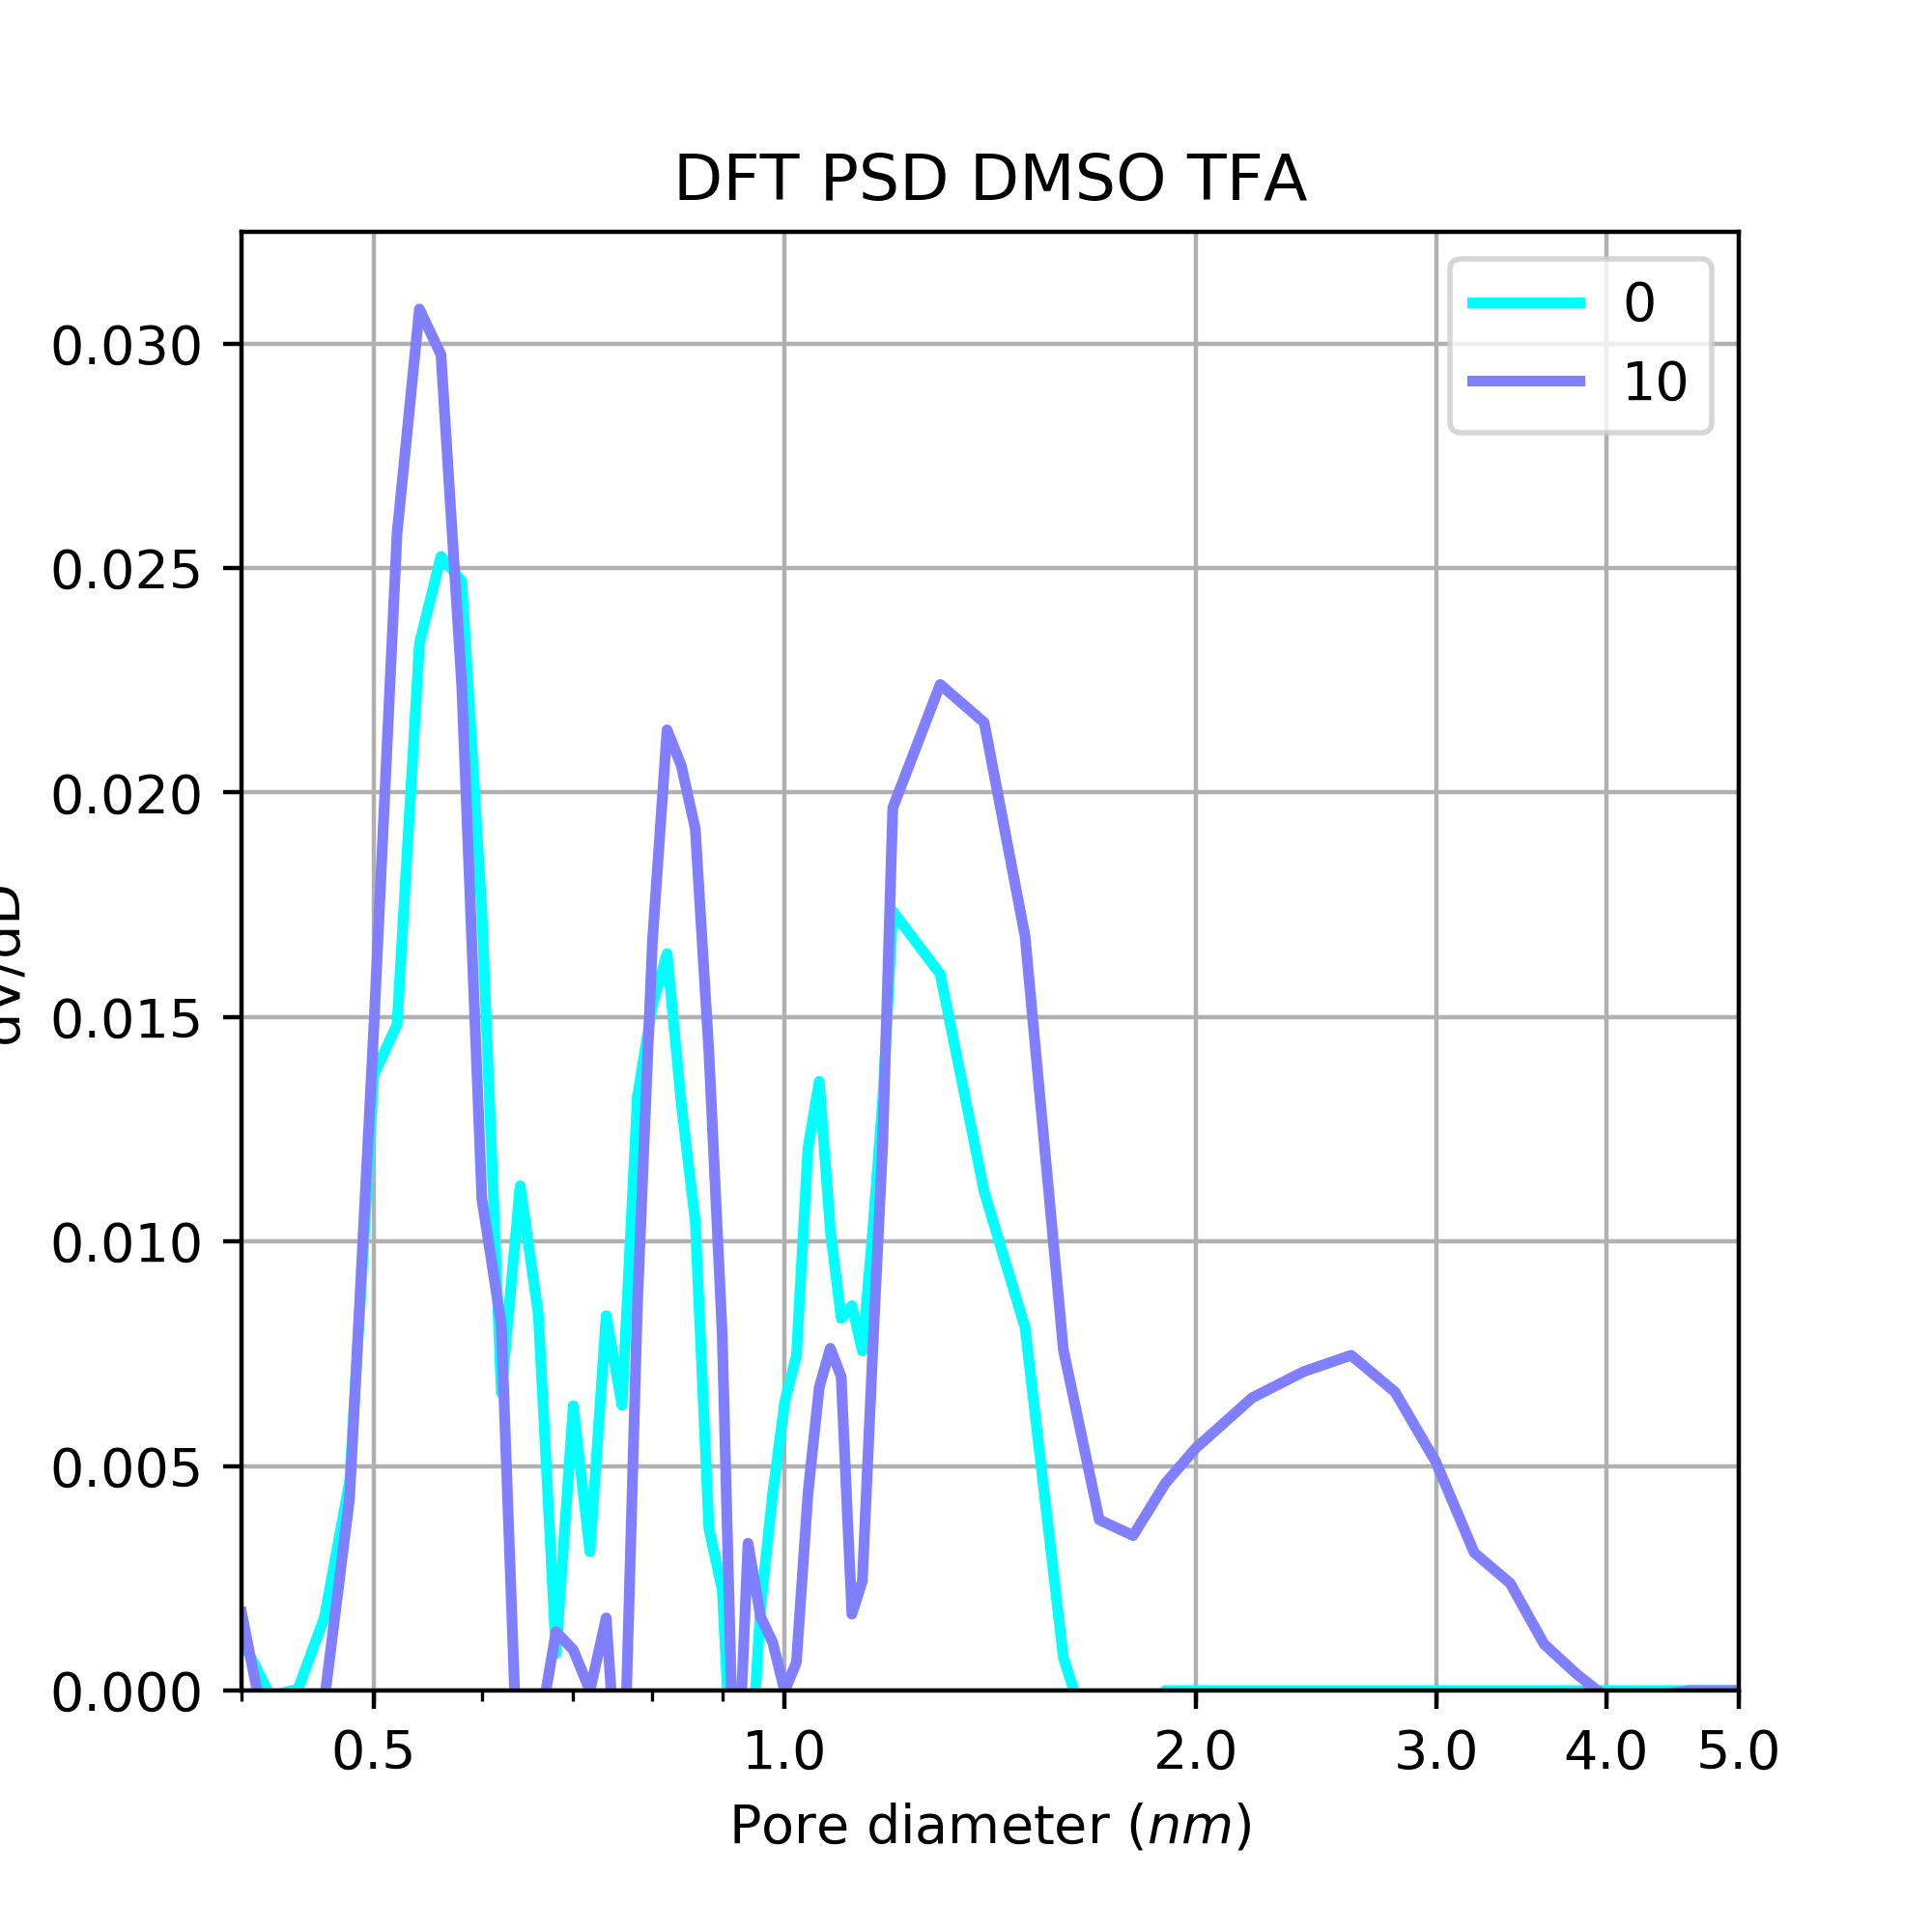
\includegraphics[width=\textwidth]{n2phys/dmso-tfa-psd-dft}%
        \label{def:fgr:psd-dmso-tfa-dft}
    \end{subfigure}%
    \begin{subfigure}{0.25\linewidth}
        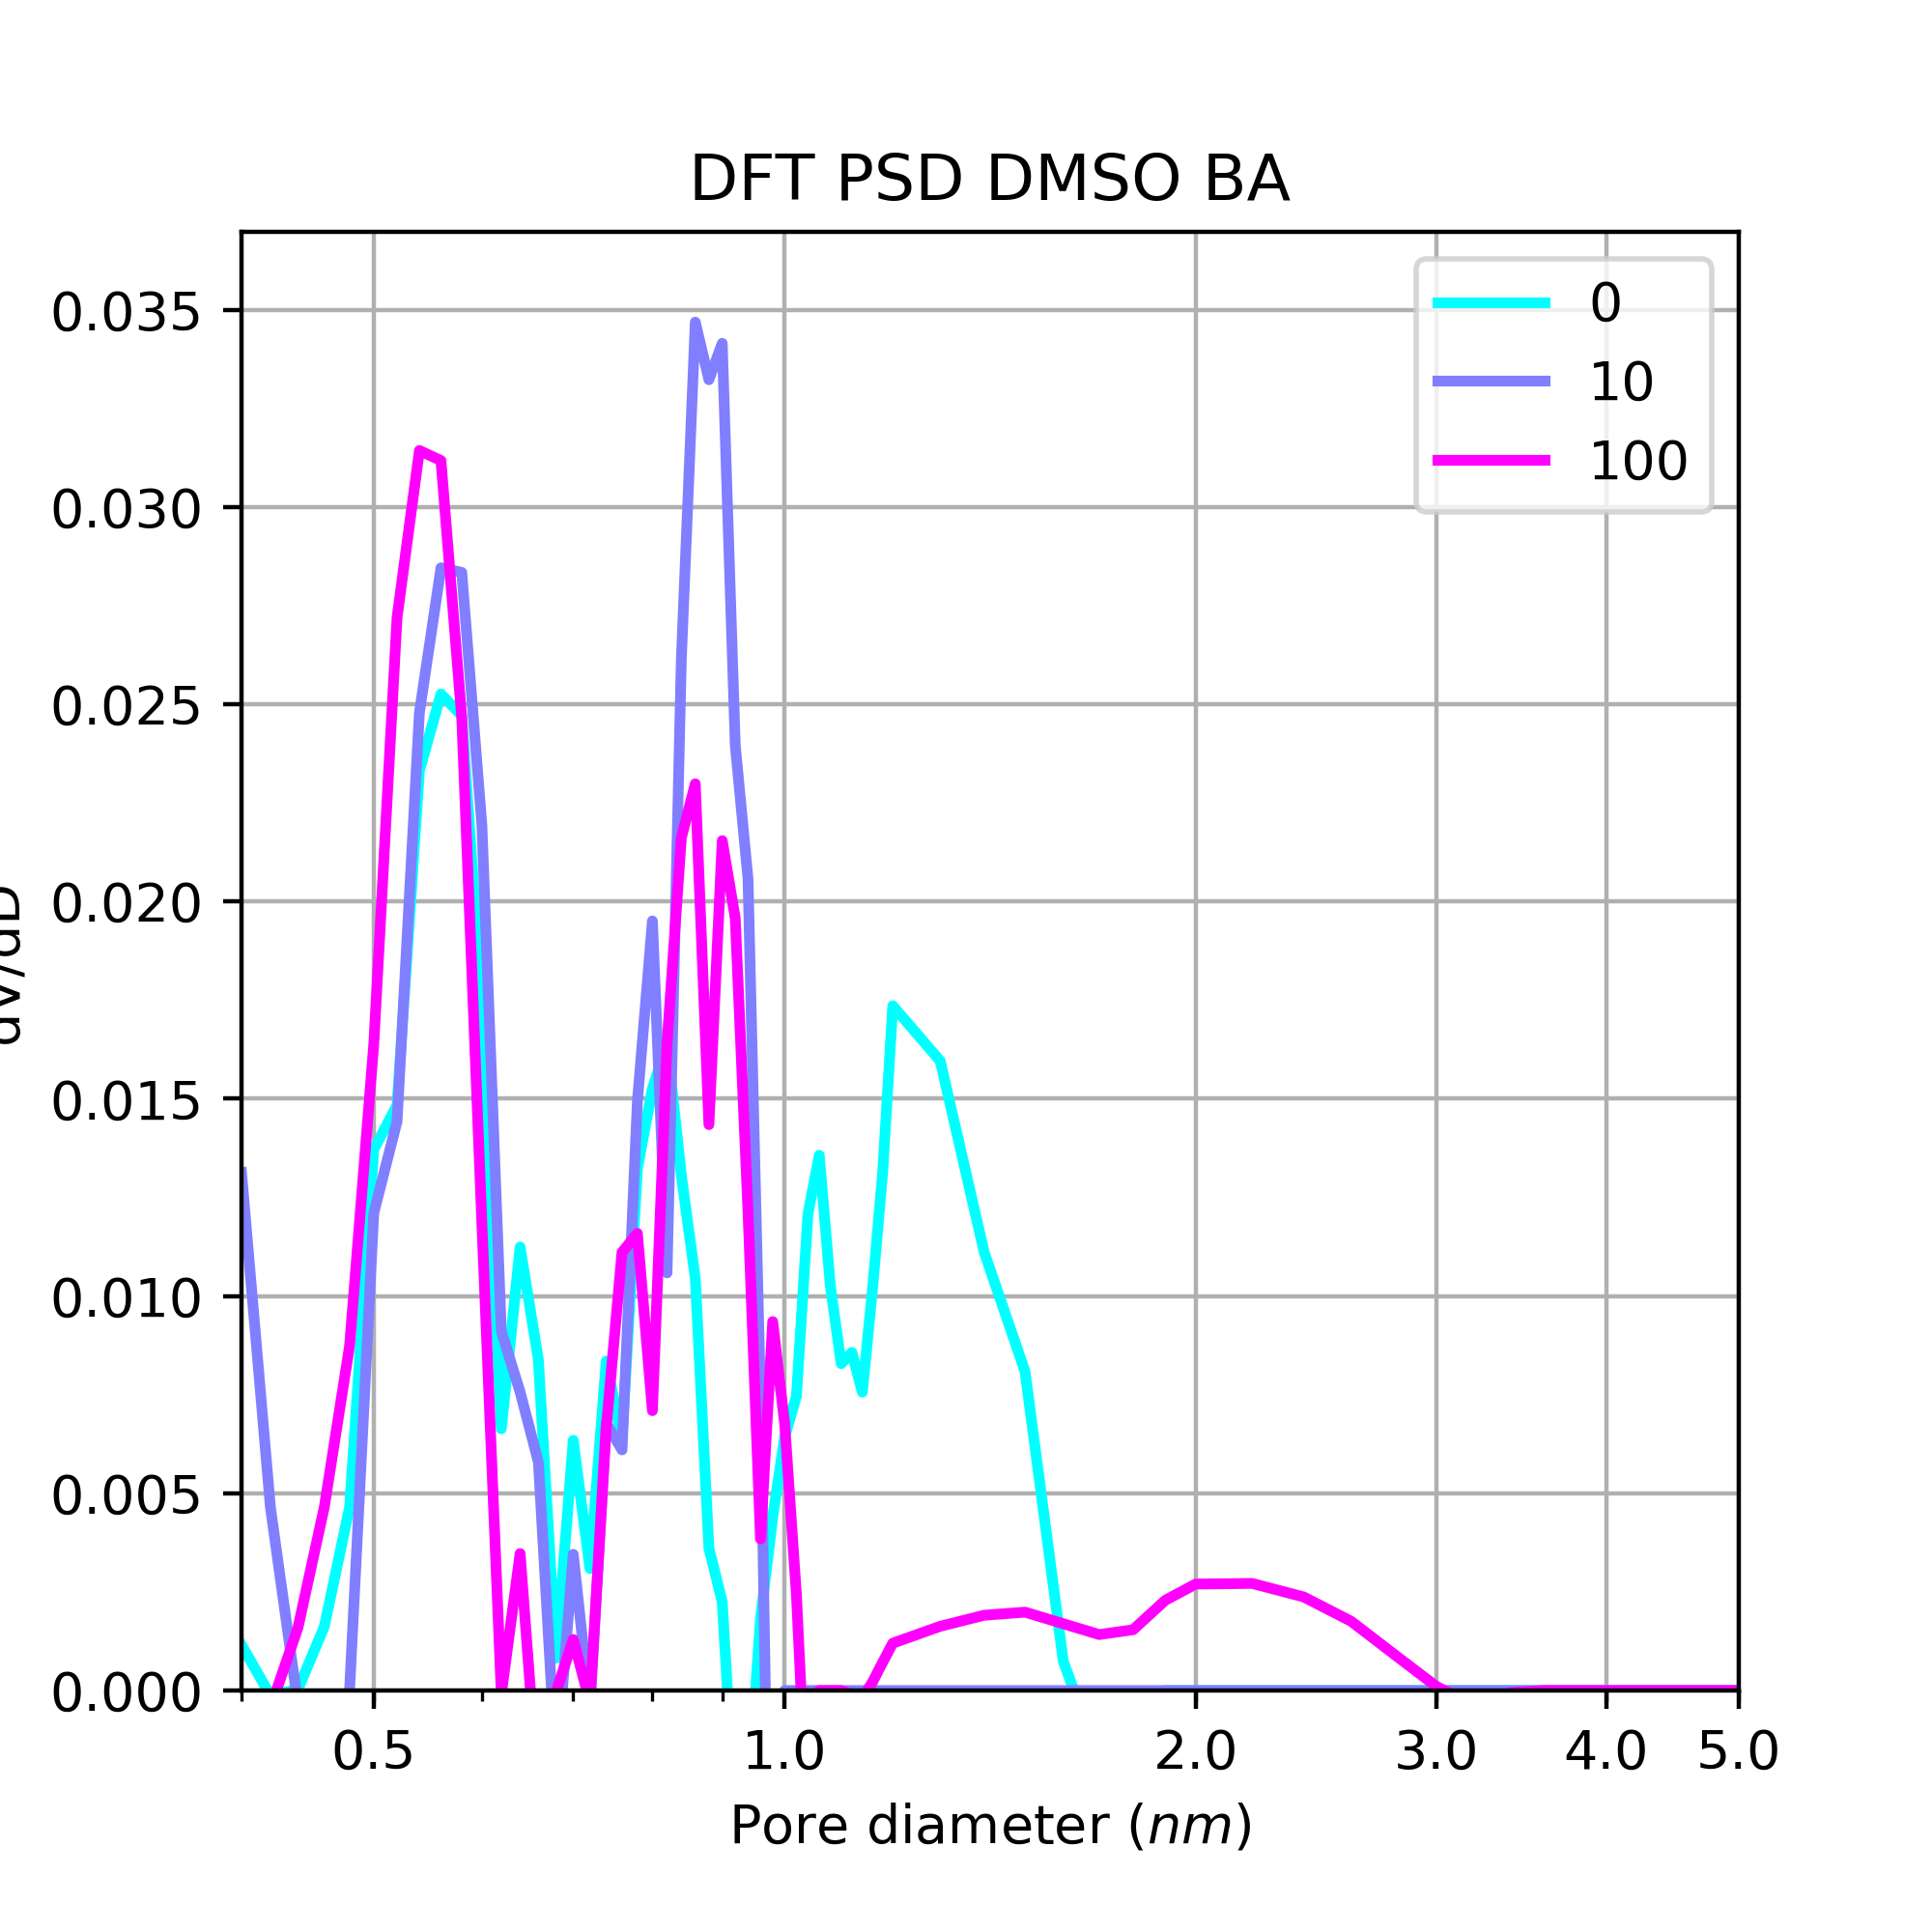
\includegraphics[width=\textwidth]{n2phys/dmso-ba-psd-dft}%
        \label{def:fgr:psd-dmso-ba-dft}
    \end{subfigure}%

    \caption{Calculated pore size distribution for the DMSO-leached
    samples with the HK (a-d) and DFT (e-h) methods.}%
    \label{def:fgr:psd}
        
\end{figure}

